% arara: xelatex: {action: nonstopmode,synctex: yes} 
% arara: biber 
% arara: xelatex: {action: nonstopmode,synctex: yes} 
% arara: xelatex: {action: nonstopmode,synctex: yes}
\RequirePackage[l2tabu, orthodox]{nag}
\documentclass[a4paper,oneside]{book}

%文献宏包 
%\usepackage[style=numeric,backend=biber]{biblatex}

\usepackage[a4paper,hscale=0.61]{geometry}
\usepackage{fontspec}

\usepackage{chngcntr}
%中文宏包
%\usepackage[UTF8,winfonts,fancyhdr,hyperref,fntef]{ctex}
\usepackage{xeCJK}

%设置字体
\setmainfont[Ligatures=TeX]{CMU Serif}
\setsansfont{CMU Sans Serif}
\setmonofont{CMU Typewriter Text}
\setCJKmainfont[BoldFont={SimHei},ItalicFont={楷体}]{SimSun}
\setCJKsansfont{Hiragino Sans GB W3}
\setCJKmonofont{幼圆}


\usepackage[svgnames]{xcolor}
\usepackage[pdfborder={0 0 0},colorlinks]{hyperref}
\usepackage{graphicx,amsmath,amssymb,bm,mathtools,subcaption,caption,cleveref}
\usepackage{mathrsfs}
\usepackage{examplep}
\usepackage{enumitem}
\usepackage{array}
\usepackage{dtklogos}
\usepackage{tablefootnote}
\usepackage{siunitx}
\usepackage[bottom]{footmisc}
\usepackage{tocloft}
\usepackage{booktabs}
\usepackage{layout}
\usepackage{cool}

%\counterwithin{chapter}{part}
%\renewcommand{\thepart}{\arabic{part}}
\makeatletter
\@addtoreset{chapter}{part}
\makeatother  

\setlength{\cftchapnumwidth}{3em}
\setlength{\cftsecnumwidth}{4em}
\setlength{\cftsubsecnumwidth}{5em}
\setlist[description]{leftmargin=6em,style=nextline,font=\normalfont}

%数学定义


%用于分隔的短横线
\newcommand{\shortline}{\noindent\rule[1mm]{30mm}{0.1mm}}

%single and double quotes
\newcommand{\sq}[1]{`#1'}
\newcommand{\dq}[1]{``#1''}

%special text
\newcommand{\coloritsf}[1]{\textcolor{cyan}{\sffamily\itshape #1}}
\newcommand{\package}[1]{\textsf{#1}}
\newcommand{\file}[1]{\textit{#1}}
\newcommand{\argument}[1]{\textit{#1}}
\newcommand{\syntax}[1]{\PVerb{#1}}
\newcommand{\envir}[1]{\PVerb{#1}}
\newcommand{\command}[1]{\PVerb{#1}}
\newcommand{\option}[1]{\PVerb{#1}}
\newcommand{\doc}[1]{\textit{#1}}

%special commands
\newcommand{\ms}[1]{$#1$\quad\PVerb{#1}}
%文献源 \addbibresource{•}


%代码宏包
\usepackage{listings}
\lstset{basicstyle=\ttfamily,frame=none,texcl=true,mathescape=true,columns=flexible,morecomment=[s][\normalfont\itshape]{<}{>},backgroundcolor=\color{Lavender},frame=single,rulecolor=\color{LightGrey}}%[latex]tex or mathematica or etc?


\title{\vspace{-20ex}\Huge\LaTeX{} Notes}
\author{Naitree Zhu}
\date{\today}

\begin{document}
\maketitle

{
  \hypersetup{linkcolor=black}% Entries in TOC are black.
  \pdfbookmark{\contentsname}{TOC}% Add bookmark for TOC in pdf.
  \tableofcontents
}

\part{General Concepts}
两类文字处理系统:
\begin{itemize}
  \item Markup language.
  \item WYSIWYG.
\end{itemize}

\paragraph{Macro}
In computer jargon, a macro is just a shorthand command that abbreviates a more complicated sequence of commands. For example, \LaTeX{}'s \command{\section} macro encodes instructions to leave some vertical space, to increment the section number counter, and to format a section heading.


\part{Basic Elements}
\chapter{换行、换页、断字}
\LaTeX{} inserts the necessary line breaks and spaces between words by optimizing the contents of a whole paragraph. If necessary, it also hyphenates words that would not fit comfortably on a line. How the paragraphs are typeset depends on the document class. Normally the first line of a paragraph is indented, and there is no additional space between two paragraphs.

\begin{lstlisting}
\\ <or> \newline
\end{lstlisting}
starts a new line but not a new paragraph.
\begin{lstlisting}
\\*
\end{lstlisting}
additionally prohibits a page break after the forced line break.

\begin{lstlisting}
\newpage
\end{lstlisting}
starts a new page.

\begin{lstlisting}
\linebreak[n], \nolinebreak[n], \pagebreak[n], \nopagebreak[n]
\end{lstlisting}
suggest places where a break may or may not happen. Optional argument \argument{n} can be set  0--4. By setting \argument{n} to a value below 4, you leave \LaTeX{} the option of ignoring your command if the result would look very bad.

when \LaTeX{} can't find a suitable place to break the line and meet its high standard, it will then let the line stick out right of the paragraph.
Then \LaTeX{} complains ``overfull hbox''. Instruct \LaTeX{} to lower its standard a little by giving \verb|\sloppy| command. It prevents over-long line by increasing inter-word spacing, even if the result is not optimal.
And in this case, a warning ``underfull hbox'' is issued. The command \verb|\fussy| brings \LaTeX{} back to its default behavior.

Sometimes it might be necessary to use \verb|\clearpage| or \verb|\cleardoublepage| to order \LaTeX{} to immediately place all floats remaining in the queues and then start a new page.

\verb|\cleardoublepage| ends the current page and causes all figures and tables that have so far appeared in the input to be printed. In a two-sided printing style, it also makes the next page a right-hand (odd-numbered) page, producing a blank page if necessary.

\begin{lstlisting}
\hyphenation{$word list$}
\end{lstlisting}
causes the words in \argument{word list} to be hyphenated only at the positions marked by hyphen `-'. No special character is allowed in the argument. For example,
\begin{lstlisting}
\hyphenation{FORTRAN Hy-phen-a-tion}
\end{lstlisting}
will allow ``hyphenation'' to be hyphenated as well as ``Hyphenation'', and it prevents ``FORTRAN'', ``Fortran'' and ``fortran'' from being hyphenated at all.
Note that the hyphenation hints are stored only for language that is active when hyphenation command occurs.

The command \verb|\-| inserts a discretionary hyphen into a word. This also becomes the only point where hyphenation is allowed in this word.

\LaTeX{} doesn't automatically hyphenate words containing special characters.

\chapter{对齐与间距}
\section{段内对齐}
段落内缺省两端对齐 (fully justified). 
另提供 3 种环境: \verb|flushleft|, \verb|flushright|, \verb|center|; 三个命令: \command{\raggedright}, \command{\raggedleft}, \command{\centering}.
\section{段首缩进与段间距}
\package{indentfirst}\\
\command{\parindent}\\
\command{\parskip}
\section{行间距}
\command{\linespread}\\
\package{setspace}
\chapter{Footnotes}
原始的脚注命令不能包含 verbatim 命令或环境.

\chapter{Margin notes}
边注可以使用 \command{\marginpar} 命令。单面排版时,边注缺省排在页面
右边空白处;双面排版时,边注在外侧,也就是左页的左边或右页的右
边;双栏页面的边注排在最近的页边。如要切换边注的方向,可以使用
\command{\reversemarginpar} 和 \command{\normalmarginpar} 命令。

\command{\marginpar} 命令使用浮动体 (float)
来生成边注,所以不能在其他浮动
体或脚注内嵌套。marginnote 宏包的 \command{\marginnote} 命令不使用浮动体,因
而没有这个缺陷。

\chapter[Hyperlinks and Cross-references]{Hyperlinks\\ and\\ Cross-references}
\section{\package{hyperref} Package}
\subsection{Commands}
\begin{description}
  \item[\syntax{\hyperref[<label>]{<text>}}] Create a link to the \syntax{<label>} in current document, with link text being the specified \syntax{<text>}.
  \item[\syntax{\url{<url>}}] Show URL in monospaced font. When the link is clicked on, a browser will open and go to that page.
  \item[\syntax{\href{<url>}{<description>}}] Show \syntax{<description>} in normal font. When it is clicked on, a browser will open and go to that page.
\end{description}
\subsection{Other forms of links}
\subsubsection{E-mail link}
Use the \syntax{mailto:} link to create link to email address.
The link has the form:
\begin{lstlisting}
mailto:<email@address.com>
\end{lstlisting}
An email address should also be present in the text. Thus incorporating the \syntax{\href} command, we get
\begin{lstlisting}[deletecomment={[s]{<}{>}}]
\href{mailto:email@address.com}{\nolinkurl{<email@address.com>}}
\end{lstlisting}

\subsubsection{Local file link}
Use the \syntax{run:} link to create link to local files.
The link has the form:
\begin{lstlisting}
run:/path/to/the/file.xxx
\end{lstlisting}
It is possible to use relative paths to link documents near the location of the current document. Use standard Unix-like notation: \syntax{./} is the current directory and \syntax{../} is the previous directory.

\subsubsection{Link anywhere in the document}
To create a targe to link to:
\begin{lstlisting}
\hypertarget{<label>}{<text>}
\end{lstlisting}
To create a link to the target:
\begin{lstlisting}
\hyperlink{<label-of-the-target>}{<text>}
\end{lstlisting}

\section{Cross-reference}
\subsection{Commands}
\begin{description}
  \item[\syntax{\label{<label>}}] A target can be labeled using the \command{\label} command if and only if it has a counter. Otherwise, not only the number will refer to the current section number, but the name will refer to the previous environment with a counter.
  \item[\syntax{\ref{<label>}}] Print the formatted number of a \syntax{<label>}.
  \item[\syntax{\pageref{<label>}}] Print the number of the page where the \syntax{<label>} is.
  \item[\syntax{\eqref{<label>}}] Provided by \package{amsmath}. It adds parentheses around the number.
  \item[\syntax{\tag{<text>}}] A tag can be manually set to replace the auto-generated number.
\end{description}

\subsection{Precautions}
In float environments, \syntax{\label} must appear inside or after \syntax{\caption}. Otherwise, it will use the current section or list number instead of what you intended.

A links to float environment will target at the caption of that environment. To make the link point to the top of the float, give the option \syntax{hypcap} to the \syntax{caption} package.


\chapter{Lists}
\chapter{Special Characters}
预定义的特殊符号见 \cref{tab:predefinedSpecial}, text mode accents 见 \cref{tab:TextModeAccents}.  
\begin{table}[htbp]
  \centering
  \begin{tabular}{ll}
    \syntax{\aa}&\aa\\
    \syntax{\AA}&\AA\\
    \syntax{\o}&\o\\
    \syntax{\textcopyright}&\textcopyright\\
    \command{\copyright}&\copyright\\
    \command{\textregistered}&\textregistered\\
    \command{\texttrademark}&\texttrademark\\
    \command{\S}&\S\\
    \command{\P}&\P\\
    \command{\pounds}&\pounds\\
    \command{\%}&\%\\
    \command{\dag}&\dag\\
    \command{\ddag}&\ddag\\
    \command{\dots}&\dots
  \end{tabular}
  \label{tab:predefinedSpecial}
  \caption{Predefined Special Characters}
  \label{tab:PredefinedSpecialCharacters}
\end{table}

\begin{table}[htbp]
  \centering
  \begin{tabular}{clclclcl}
    \toprule
    \.{a}&\command{\.{a}}&\"{a}&\command{\"{a}}&\={a}&\command{\={a}}&\`{a}&\command{\`{a}}\\
    \'{a}&\command{\'{a}}&\v{a}&\command{\v{a}}&\^{a}&\command{\^{a}}&\~{a}&\command{\~{a}}\\
    \d{a}&\command{\d{a}}&\b{a}&\command{\b{a}}&\r{a}&\command{\r{a}}&&\command{\textcircled{a}}\\
    \bottomrule
  \end{tabular}
  \caption{Text mode accents.}
  \label{tab:TextModeAccents}
\end{table}


\begin{table}
  \centering
  The following symbols can be negated by prefixing them with a \verb|\not| command.\\
  \medskip
  \begin{tabular}{ll}
    \ms{\leq} or \verb|\le|&\ms{\geq} or \verb|\ge|\\
    \ms{\leqslant}&\ms{\geqslant}\\
    \ms{\ll}&\ms{\gg}\\
    \ms{\equiv}&\ms{\triangleq}\\
    \ms{\subset}&\ms{\supset}\\
    \ms{\approx}&\\
    \ms{\subseteq}&\ms{\supseteq}\\
    \ms{\subseteqq}&\ms{\supseteqq}\\
    \ms{\cong}&\\
    \ms{\in}&\ms{\ni} or \verb|\owns|\\
    \ms{\propto}&\ms{\varpropto}\\
  \end{tabular}

  The followings are negated Binary relation symbols.\\
  \medskip
  \begin{tabular}[c]{ll}
    \ms{\notin}&\ms{\neq} or \verb|\ne|\\
    \ms{\nless}&\ms{\ngtr}\\
    \ms{\lneq}&\ms{\gneq}\\
    \ms{\nleq}&\ms{\ngeq}\\
    \ms{\nleqslant}&\ms{\ngeqslant}\\
    \ms{\subsetneq}&\ms{\supsetneq}\\
    \ms{\nsubseteq}&\ms{\nsupseteq}\\
    \ms{\subsetneqq}&\ms{\supsetneqq}\\
    \ms{\nsubseteqq}&\ms{\nsupseteqq}\\
  \end{tabular}
  \caption{Binary Relations}
  \label{tab:binaryrelations}
\end{table}

\begin{table}
  \centering
  \begin{tabular}{ll}
    \ms{\pm}&
    \ms{\mp}\\
    \ms{\div}&\\
    \ms{\oplus}&
    \ms{\otimes}\\
    \ms{\dagger}&
    \ms{\ddagger}\\
    \ms{\cup}&\ms{\cap}\\
    \ms{\setminus}&\\
    \ms{\circ}&\\
  \end{tabular}
  \caption{Binary Operators}
  \label{tab:binaryoperator}
\end{table}

\begin{table}
  \centering
  \begin{tabular}{l}
    \ms{\sum}\\
    \ms{\prod}\\
    \ms{\int}\\
    \ms{\bigoplus}\\
    \ms{\bigcup}\\
    \ms{\bigcap}\\
    \ms{\oint}\\
    \ms{\bigotimes}
  \end{tabular}
  \caption{Big Operators}
  \label{tab:bigoperators}
\end{table}

\begin{table}
  \centering
  \begin{tabular}{lp{5cm}}
    \ms{\leftarrow} or \verb|\gets|&\ms{\longleftarrow}\\
    \ms{\rightarrow} or \verb|\to|&\ms{\longrightarrow}\\
    \ms{\leftrightarrow}&\ms{\longleftrightarrow}\\
    \ms{\Leftarrow}&\ms{\Longleftarrow}\\
    \ms{\Rightarrow}&\ms{\Longrightarrow}\\
    \ms{\Leftrightarrow}&\ms{\Longleftrightarrow}\\
    \ms{\mapsto}&\ms{\longmapsto}\\
    \ms{\hookleftarrow}&\ms{\hookrightarrow}\\
    \ms{\leftharpoonup}&\ms{\rightharpoonup}\\
    \ms{\leftharpoondown}&\ms{\rightharpoondown}\\
    \ms{\rightleftharpoons}&\ms{\iff} (bigger spaces than \verb|\Longleftrightarrow|)\\
    \ms{\uparrow}&\ms{\downarrow}\\
    \ms{\updownarrow}&\ms{\Uparrow}\\
    \ms{\Downarrow}&\ms{\Updownarrow}\\
    \ms{\nearrow}&\ms{\searrow}\\
    \ms{\swarrow}&\ms{\nwarrow}\\
    \ms{\leadsto} (\package{latexsym} package)&\\
    \ms{\dashleftarrow}&\ms{\dashrightarrow}\\
    \ms{\leftleftarrows}&\ms{\rightrightarrows}\\
    \ms{\leftrightarrows}&\ms{\rightleftarrows}\\
    \ms{\Lleftarrow}&\ms{\Rrightarrow}\\
    \ms{\twoheadleftarrow}&\ms{\twoheadrightarrow}\\
    \ms{\leftarrowtail}&\ms{\rightarrowtail}\\
    \ms{\leftrightharpoons}&\ms{\rightleftharpoons}\\
    \ms{\curvearrowleft}&\ms{\curvearrowright}\\
    \ms{\circlearrowleft}&\ms{\circlearrowright}\\
    \ms{\upuparrows}&\ms{\downdownarrows}\\
    \ms{\upharpoonleft}&\ms{\upharpoonright}\\
    \ms{\downharpoonleft}&\ms{\downharpoonright}\\
    \ms{\nleftarrow}&\ms{\nrightarrow}\\
    \ms{\nleftrightarrow}&\\
    \ms{\nLeftarrow}&\ms{\nRightarrow}\\
    \ms{\nLeftrightarrow}&\\
  \end{tabular}
  \caption{Arrows}
  \label{tab:arrows}
\end{table}

\begin{table}
  \centering
  \begin{tabular}{ll}
    \ms{\overrightarrow{AB}}&\ms{\underrightarrow{AB}}\\
    \ms{\overleftarrow{AB}}&\ms{\underleftarrow{AB}}\\
    \ms{\overleftrightarrow{AB}}&\ms{\underleftrightarrow{AB}}
  \end{tabular}
  \caption{Arrows as Accents}
  \label{tab:arrowsAccent}
\end{table}

\begin{table}
  \centering
  \begin{tabular}{ll}
    \ms{[} or \verb|\lbrack|&\ms{]} or \verb|\rbrack|\\
    \ms{\{} or \verb|\lbrace|&\ms{\}} or \verb|\rbrace|\\
    \ms{\langle}&\ms{\rangle}\\
    \ms{\lvert}&\ms{\rvert}\\
    $\vert$\quad\verb+|+ or \verb|\vert|&\ms{\|} or \verb|\Vert|\\
    \ms{\lVert}&\ms{\rVert}\\
    \ms{/}&\ms{\backslash}\\
    \ms{\lfloor}&\ms{\rfloor}\\
    \ms{\lceil}&\ms{\rceil}\\
    \ms{\ulcorner}&\ms{\urcorner}\\
    \ms{\llcorner}&\ms{\lrcorner}\\
    \ms{\uparrow}&\ms{\downarrow}\\
    \ms{\Uparrow}&\ms{\Downarrow}\\
    \ms{\updownarrow}&\ms{\Updownarrow}
  \end{tabular}
  \caption{Delimiters}
  \label{tab:delimiters}
\end{table}

\begin{table}
  \centering
  \begin{tabular}{ll}
    \ms{\dots}&\ms{\cdots}\\
    \ms{\vdots}&\ms{\ddots}\\
    \ms{\hbar}&\ms{\hslash}\\
    \ms{\exists}&\ms{\nexists}\\
    \ms{\forall}&\\
    \ms{'}&\ms{\prime}\\
    \ms{\bot}&\ms{\angle}\\
    \ms{\surd}&\ms{\neg} or \verb|\lnot|\\
    \ms{\sharp}&\ms{\triangle}\\
    \ms{\emptyset}&\ms{\varnothing}\\
    \ms{\because}&\ms{\therefore}\\
    \ms{\square}&\ms{\blacksquare}\\
    \ms{\angle}&\ms{\measuredangle}\\
  \end{tabular}
  \caption{Miscellaneous Symbols}
  \label{tab:miscSymbols}
\end{table}

\part{Document Structure}
标题、目录、正文、参考文献、索引.
\chapter{长文档}
\begin{verbatim}
\include{filename}
\end{verbatim}
to insert contents of another \TeX{} file. note that \LaTeX{} will start a new page before processing \file{filename.tex}.

\begin{verbatim}
\includeonly{filename1,filename2,...}
\end{verbatim}
after this command is executed in the preamble of the document, only \verb|\include| commands for the filenames that are listed in the argument of the \verb|\includeonly| command will be executed.

\begin{verbatim}
\input{filename}
\end{verbatim}
simply includes the file specified, without page breaks or any other effects.

在长文档中使用参考文献时, 用 latex 编译主控文档, bibtex 编译子文档.

\chapter{Bibliography}
If using BibTeX, the best way of inserting accented characters(and other similar stuffs) is of the form: \verb|{\'o}|. Whereas, if using biber, normal \verb|\'{o}| would work fine.
\chapter{Index}
Progress \verb|.idx| file through program \verb|makeindex| to generate \verb|.ind| file, which will be progressed by \LaTeX{} to print Index.

Procedures for index generation.
\begin{enumerate}
  \item Load \package{makeidx} package in the preamble.
  \item Put the command \verb|\makeindex| in the preamble to enable special indexing commands.
  \item Type the index command
    \begin{lstlisting}
    \index{$key$@$formatted$_$entry$}
    \end{lstlisting}
    at the point where you want the final index entry to point to. $formatted$\verb|_|$entry$ will appear in the index and $key$ will be used for sorting.
    The $formatted$\verb|_|$entry$ is optional. If it is missing, the $key$ will be printed.
\end{enumerate}

When the input file is processed with \LaTeX{}, each \verb|\index| command writes an corresponding index entry, together with the current page number, to a special file (\verb|.idx| file). This \verb|.idx| file will then be processed with the \verb|makeindex| program to generates a sorted index file (\verb|.ind| file). Then process the input file again with \LaTeX{}. This sorted index will get included into the document at the point where the command
\begin{lstlisting}
\printindex
\end{lstlisting}
appears.

Examples of \verb|\index| command usage are shown in \cref{tab:indexcommand}.
\begin{table}[htbp]
  \centering
\begin{tabular}[]{lll}
  \textbf{Example}&\textbf{Index Entry}&\textbf{Comment}\\
  \hline
  \verb|\index{hello}|&hello, 1&Plain entry\\
  \verb|\index{hello!Peter}|&\quad Peter, 3&Subentry under \sq{hello}\\
  \verb|\index{Lin@\\textbf{Lin}}|&\textbf{Lin}, 7&Formatted entry\\
  \verb|\index{Kaese@K\"ase}|&K\"{a}se, 33&Formatted entry\\
  \verb+\index{Jenny|textbf}+&Jenny, \textbf{3}&Formatted page number
\end{tabular}
\caption{index command usage}
\label{tab:indexcommand}
\end{table}
For systematic explanation of syntax used in \verb|\index| command, please read the \verb|makeindex.dvi| documentation. 

\verb|makeindex| has no clue about characters outside the ASCII range. To get the sorting correct, use the \verb|@| to specify (and delimit) a sorting key.

\part{Layouts}
\chapter{Page Dimensions}
\section{\LaTeX{} Native Dimensions}
\layout

页面右边距和下边距都是设置其他长度后剩出来的.

\command{\oddsidemargin} 和 \command{\evensidemargin} 指的是奇数页和偶数页的左边距.

\section{\package{geometry} package}
\begin{center}
  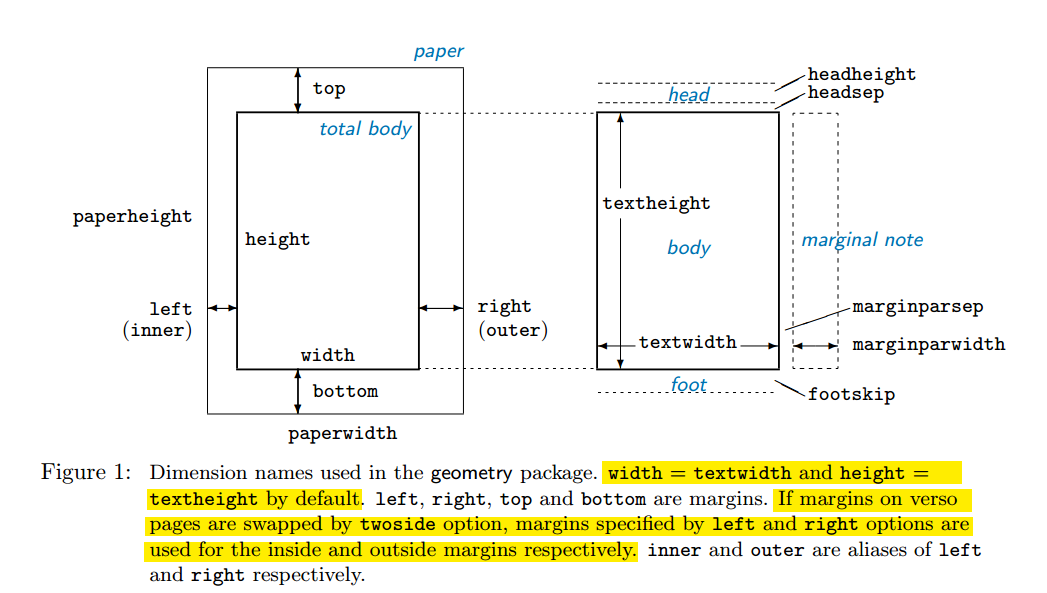
\includegraphics[width=0.99\textwidth]{geometry_figure_1}
  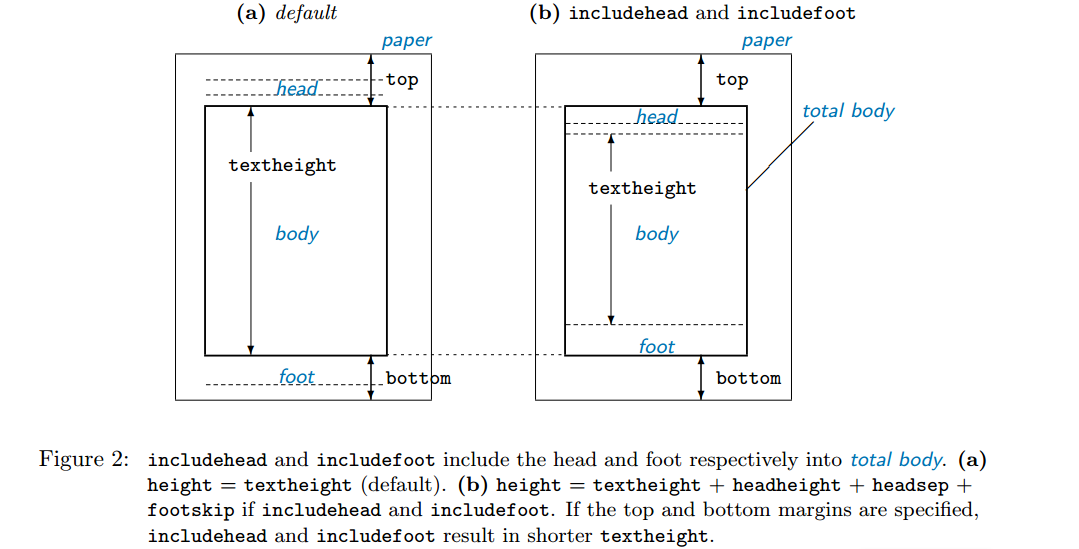
\includegraphics[width=0.99\textwidth]{geometry_figure_2}
\end{center}

\begin{table}[htpb]
\noindent\begin{tabular}[h]{|rcp{9cm}|}
  \hline
\coloritsf{paper}&:&\coloritsf{total body} and \coloritsf{margins}\\
\coloritsf{total body}&:&\coloritsf{body} (main text area) (with optional \coloritsf{header}, \coloritsf{footer} and \coloritsf{marginal notes part})\\
\coloritsf{margin}&:&\coloritsf{left} (\coloritsf{inner}), \coloritsf{right} (\coloritsf{outer}), \coloritsf{top} and \coloritsf{bottom}\\
\hline
\end{tabular}
\end{table}

Obviously, \coloritsf{inner} and \coloritsf{outer} margins are for two--sided document. Each margin is measured from the corresponding edge of a paper.

The dimensions for \coloritsf{paper}, \coloritsf{total body} and \coloritsf{margins} have the following relations.
\begin{align}
  \texttt{paperwidth}&=\texttt{left}+\texttt{width}+\texttt{right}\\
  \texttt{paperheight}&=\texttt{top}+\texttt{height}+\texttt{bottom}
\end{align}

The \coloritsf{total body} width and height are defined:
\begin{align}
  \texttt{width}&=\texttt{textwidth}(+\texttt{marginparsep}+\texttt{marginparwidth})\\
  \texttt{height}&=\texttt{textheight}(+\texttt{headheight}+\texttt{headsep}+\texttt{footskip})
\end{align}

\texttt{width=textwidth} by default, while \texttt{marginparsep} and \texttt{marginparwidth} are included in \texttt{width} if \texttt{includemp} option is set \texttt{true}. \texttt{height:=textheight} by default. If \texttt{includehead} is set to true, \texttt{headheight} and \texttt{headsep} are considered as a part of \texttt{height}. In the same way, \texttt{includefoot} takes \texttt{footskip} into \texttt{height}.

\subsection{Commands}

\begin{verbatim}
\geometry{options}
\newgeometry{options}
\restoregeometry
\savegeometry{name}
\loadgeometry{name}
\end{verbatim}

Options for \verb|\usepackage|, \verb|\geometry| and \verb|\newgeometry| are comma-separated using \textsf{keyval} interface.

\subsection{Rules of options}

Multiple lines are allowed, while blank lines are not.
Any spaces between words are ignored.
Options are basically order-independent. (With certain exceptions.)
Some options allow sublist.

Multiple use of \verb|\geometry| just appends options.

\subsection{Type of options}

\subsubsection{Boolean:}
\begin{verbatim}
<key>=true|false
<key> without value equals to value true
\end{verbatim}

\subsubsection{Single-valued:}
\begin{verbatim}
<key>=<value>
\end{verbatim}

\subsubsection{Double-valued:}
\begin{verbatim}
<key>={<value1>,<value2>}
<key>=<value> equals to <key>={<value>,<value>}
\end{verbatim}

\subsubsection{Triple-valued:}
\begin{verbatim}
<key>={<value1>,<value2>,<value3>}
\end{verbatim}

When you give an empty value or `*', it means null and leaves the appropriate value to the auto-completion mechanism. You need to specify at least one dimension, typically two dimensions.

\subsection{Option Details}
\emph{Note}: options with a marked dagger ($\dag$) are not available to \verb|\newgeometry|.

\subsubsection{Options for paper}

\paragraph{$\dag$\texttt{paper}} specifies the paper size by name. Paper name can be specified without \verb|paper=|\,.

\paragraph{$\dag$\texttt{a[0-6]paper, b[0-6]paper, c[0-6]paper, b[0-6]j,ansi[a,b,c,d,e]paper,\\ letterpaper, executivepaper, legalpaper}}\hfill\\
specify paper name. Value part is ignored even if any.
\texttt{a[0-6]paper}, \texttt{b[0-6]paper}, \texttt{c[0-6]paper} are ISO A, B and C series of paper sizes respectively. The JIS (Japanese Industrial Standards) A-series is identical to the ISO A-series, but the JIS B-series is different from the ISO B-series. \texttt{b[0-6]j} should be used for the JIS B-series.

\paragraph{$\dag$\texttt{screen}} a special paper size with (W,H) = (225mm,180mm). For presentation with PC and video projector, ``\texttt{screen,centering}'' with `\texttt{slide}' documentclass would be useful.

\paragraph{$\dag$\texttt{paerwidth}} the width of paper.

\paragraph{$\dag$\texttt{paperheight}} the height of paper.

\paragraph{$\dag$\texttt{papersize}} \verb|papersize={<width>,<height>}|, or \verb|papersize=<length>|.

\paragraph{$\dag$\texttt{landscape}}: switch paper orientation to landscape.

\paragraph{$\dag$\texttt{portrait}} switch to portrait, equivalent to \texttt{landscape=false}.

The options for paper names (e.g., \texttt{a4paper}) and orientation (\texttt{portrait} and \texttt{landscape}) can be set as documentclass options. For example, if you set \begin{verbatim}\documentclass[a4paper,landscape]{article}\end{verbatim} then \texttt{a4paper} and \texttt{landscape} are processed in \textsf{geometry} as well. This also the case for \texttt{twoside} and \texttt{twocolumn}.

\subsubsection{Options for total body}
\begin{description}
  \item[\syntax{hscale}] ratio of \texttt{width} of \coloritsf{total body} to \verb|\paperwidth|. Default $0.7$.

  \item[\syntax{vscale}] ratio of \texttt{height} of \coloritsf{total body} to \verb|\paperheight|. Default $0.7$.

  \item[\syntax{scale}] \verb|scale={<hscale>,<vscale>}|, or \verb|scale=<scale>|. Default $0.7$.

  \item[\syntax{width}] \texttt{width} of \coloritsf{total body}. \verb|width=<length>|. This dimension defaults to \texttt{textwidth}, but if \texttt{includemp} is set to \texttt{true}, then \texttt{width} $\geqslant$ \texttt{textwidth} because \texttt{width} includes the width of the marginal notes.

  \item[\syntax{height}] height of \coloritsf{total body}, excluding header and footer by default. If \texttt{includehead} or \texttt{includefoot} is set, \texttt{height} includes the head or foot of the page as well as \texttt{textheight}.

  \item[\syntax{total}] width and height of \coloritsf{total body}. \lstinline[breaklines]|total={<width>,<height>}|, or \lstinline[breaklines]|total=<length>|.

  \item[\syntax{textwidth}] the width of \coloritsf{body} (text area).

  \item[\syntax{textheight}] the height of \coloritsf{body} (text area).

  \item[\syntax{text}] width and height of \coloritsf{body}. \verb|text={<width>,<height>}|, or \lstinline[breaklines]|text=<length>|.

  \item[\syntax{lines}] specify \verb|\textheight| by number of lines. \verb|lines=<integer>|.

  \item[\syntax{includehead}] includes \verb|\headheight| and \verb|\headsep| into \coloritsf{total body}. Default \texttt{false}.

  \item[\syntax{includefoot}] includes \verb|\footskip| into \coloritsf{total body}. Default \texttt{false}.

  \item[\syntax{includeheadfoot}] set both above.

  \item[\syntax{includemp}] includes \verb|\marginparwidth| and \verb|\marginparsep| into \coloritsf{body}.

  \item[\syntax{includeall}] include all three parts above into \coloritsf{total body}.

  \item[\syntax{ignorehead}] excludes the head from \coloritsf{total body}. Default \verb|true|.

  \item[\syntax{ignorefoot}] Default \texttt{true}.

  \item[\syntax{ignoreheadfoot}] Default \texttt{true}.

  \item[\syntax{ignoremp}] Default \texttt{true}.

  \item[\syntax{ignoreall}] Default \texttt{true}.
\end{description}
\subsubsection{Options for partition}
\begin{description}
  \item[\syntax{hdivide}] specify the length of three parts simultaneously. \lstinline[breaklines]|hdivide={<left-margin>,<width>,<right-margin>}|. Note that the best way is to leave one of them empty or marked with `*'.

  \item[\syntax{vdivide}] as above.

  \item[\syntax{divide}] \verb|divide={A,B,C}| is interpreted as \verb|hdivide=vdivide={A,B,C}|.
\end{description}
\subsubsection{Options for margin}
\begin{description}
\item[\syntax{left|inner}] the distance between left (inner) edge of paper and that of \coloritsf{total body}.

\item[\syntax{right|outer}] as above.

\item[\syntax{top}] as above.

\item[\syntax{bottom}] as above.

\item[\syntax{hmargin}] \verb|hmargin={<left>,<right>}|, or \verb|hmargin=<length>|.

\item[\syntax{vmargin}] \verb|vmargin={<top>,<bottom>}|, or \verb|<length>|.

\item[\syntax{margin}] \verb|margin={A,B}| is equivalent to \verb|hmargin={A,B}| and \verb|vmargin={A,B}|. \verb|margin=A| equals to \verb|hmargin=A| and \verb|vmargin=A|.

\item[\syntax{hmarginratio}] horizontal margin ratio of \texttt{left} (\texttt{inner}) to \texttt{right} (\texttt{outer}). The value should be specified with colon-separated two values. Each value should be a positive integer less than 100 to prevent arithmetic overflow. Default $1:1$ for oneside, $2:3$ for twoside.

\item[\syntax{vmarginratio}] ratio of \verb|top| to \verb|bottom|. Default $2:3$.

\item[\syntax{marginratio}] \lstinline|marginratio={<hmarginratio>,<vmarginratio>}|, or \lstinline[breaklines]|marginratio=<ratio>|.

\item[\syntax{hcentering}] sets horizontal centering. It is equivalent to \verb|hmarginratio=1:1|. Default \verb|true| for oneside.

\item[\syntax{vcentering}] Default \verb|false|.

\item[\syntax{centering}] sets both horizontal and vertical centering. Default \verb|false|.

\item[\syntax{twoside}] switches on twoside mode with left and right margins swapped on verso pages.

\item[\syntax{bindingoffset}] removes a specified space from the lefthand-side of the page for oneside or the inner-side for twoside. \verb|bindingoffset=<length>|.
\end{description}

\subsubsection{Options for Native \LaTeX{} Dimensions}
\begin{description}
\item[\syntax{headheight}] modifies \verb|\headheight|, height of header. \verb|headheight=<length>|.

\item[\syntax{headsep}] modifies \verb|\headsep|, separation between header and main text area (\coloritsf{body}). \lstinline[breaklines]|headsep=<length>|.

\item[\syntax{footskip}] modifies \verb|\footskip|, separation between baseline of last line of text and baseline of footer.

\item[\syntax{nohead}] eliminates spaces for head of page, equivalent to both \lstinline[breaklines]|\headheight=0pt| and \verb|\headsep=0pt|.

\item[\syntax{nofoot}] eliminates spaces for foot of page, equivalent to \verb|\footskip=0pt|.

\item[\syntax{noheadfoot}] sets both \texttt{nohead} and \texttt{nofoot}.

\item[\syntax{footnotesep}] changes the dimension \verb|\skip\footins|, separation between the bottom of text body and the top of footnote text.

\item[\syntax{marginparwidth}] modifies \verb|\marginparwidth|, width of the marginal notes.

\item[\syntax{marginparsep}] modifies \verb|\marginparsep|, separation between main text area (\coloritsf{body}) and marginal notes.

\item[\syntax{nomarginpar}] shrinks spaces for marginal notes to 0pt, equivalent to both \verb|\margin| \verb|parwidth=0pt| and \verb|\marginparsep=0pt|.

\item[\syntax{columnsep}] modifies \verb|\columnsep|, separation between two columns in \verb|twocolumn| mode.

\item[\syntax{twocolumn}] sets \texttt{twocolumn} mode. \verb|twocolumn=false| is equivalent to \verb|onecolumn|.

\item[\syntax{onecolumn}] \verb|onecolumn=false| is equivalent to \verb|twocolumn|.

\item[\syntax{reversemp}] makes the marginal notes appear in the left (inner) margin. Default \texttt{false}.
\end{description}

\subsubsection{Options for Drivers}
By default, \textsf{geometry} package guesses the driver appropriate to the system in use. Therefore, you don't have to set a driver in most cases.


\subsection{Processing}
\subsubsection{Order of loading}
The order of loading in the preamble is as follows:
\begin{enumerate}
  \item \verb|geometry.cfg| if exists.
  \item Options specified with \verb|documentclass[options]{...}|
  \item Options specified with \verb|\usepackage[options]{geometry}|
  \item Options specified with \verb|\geometry{options}|, which can be called multiple times. (Option \texttt{reset} will cancel the specified options ever given in command \verb|\usepackage{geometry}| or \verb|\geometry|.)
\end{enumerate}

\subsubsection{Order of options}
The specification of \textsf{goemetry} options is order-independent, and overwrites the previous one for the same setting. 

For example, \verb|[hmargin={3cm,2cm},left=1cm]| equals to \verb|hmargin={1cm,2cm}|.

\texttt{reset} and \texttt{mag} are exceptions. The \texttt{reset} option removes all the geometry options (except \texttt{pass}) before it.
\subsubsection{Priority}
There are several ways to set dimensions of the \coloritsf{body} : \texttt{scale}, \texttt{total}, \texttt{text} and \texttt{lines}. The \textsf{geometry} package gives higher priority to the more concrete specification.
\[
  \texttt{lines} 
  > 
  \left\{
    \begin{aligned}
      &\texttt{textwidth}\\
      &\texttt{textheight}\\
      &\texttt{text}
    \end{aligned}
  \right\}
  >
  \left\{ 
    \begin{aligned}
      &\texttt{width}\\
      &\texttt{height}\\
      &\texttt{total}
    \end{aligned}
  \right\}
  >
  \left\{ 
    \begin{aligned}
      &\texttt{hscale}\\
      &\texttt{vscale}\\
      &\texttt{scale}
    \end{aligned}
  \right\}
\]

\subsubsection{Defaults}

The default vertical margin ratio is 2/3, namely,
\[
  \texttt{top}:\texttt{bottom}=2:3
\]

The default horizontal margin ratio, is specified with \verb|oneside| and \verb|twoside| respectively,
\[
  \texttt{left}(\texttt{inner}):\texttt{right}(\texttt{outer})=\left\{\begin{aligned}
    1:1&\qquad \text{default for \texttt{oneside}}\\
    2:3&\qquad \text{default for \texttt{twoside}}
  \end{aligned}\right.
\]

The default horizontal margin ratio for oneside is \sq{centering}.

The \textsf{geometry} package has the following default setting for \emph{onesided} document:
\begin{itemize}
  \item \texttt{scale}=0.7 
  \item \verb|marginratio={1:1,2:3}|
  \item \verb|ignoreall|
\end{itemize}
For \emph{twosided} document, the default setting is the same as \emph{oneside} except that the horizontal margin ratio is set to \verb|2:3|.

\chapter{Page Styles}
Native \LaTeX{} supports two commands to change page style(header and footer).

The \verb|\pagestyle| command apply the specified style to the current and all subsequent pages.

\verb|\thispagestyle| will only affect the page where the command is inserted.

The possible styles are:

\begin{tabular}[h]{lp{8cm}}
  \texttt{empty} & no header and footer\\
  \texttt{plain} & no header, footer contains page number in the center\\
  \texttt{headings} & Footer is blank, header displays information according to document class (e.g., section name) and page number top right.\\
  \texttt{myheadings} & page numbers is top right, other commands can be provided to control the rest of header.
\end{tabular}

With \verb|myheadings|, the commands \verb|\markright|(in the standard documents class: article, report and book) and \verb|\markboth| (in the book class) are used to control the headings.

For example,
\begin{lstlisting}
\pagestyle{myheadings}
\markright{A\hfill B\hfill}
\end{lstlisting}
will place A to the top left, B to the top centered and page number to the top right, for every page from the current page on.

\section{Using \textsf{fancyhdr} package}
With \textsf{fancyhdr} package, a new page style \verb|fancy| is now available:
\begin{lstlisting}
\pagestyle{fancy}
\end{lstlisting}

Following the \verb|\pagestyle| command are six commands which define the behaviors of six respective areas in header and footer. 

\begin{verbatim}
\lhead{}
\chead{}
\rhead{}
\lfoot{}
\cfoot{}
\rfoot{}
\end{verbatim}

In each of the command above, add text or commands.

Some useful commands including:

\begin{tabular}[h]{lp{8cm}}
  \verb|\thepage| & number of the current page\\
  \verb|\thechapter| & current chapter number\\
  \verb|\thesection| & current section number\\
  \verb|\leftmark| & current chapter name printed like:
  \begin{center}
    CHAPTER X.~CHAPTER TITLE 
  \end{center}\\
  \verb|\rightmark| & current section name printed like: 
  \begin{center}
  X.~X.~SECTION TITLE
\end{center}\\
  \verb|\chaptername| & the name of the chapter in the current language, like:
  \begin{center}
    Chapter Name
  \end{center}
\end{tabular}

\emph{Note}: The standard \LaTeX~classes have the command \verb|\maketitle| defined in such a way that \verb|\thispagestyle{plain}| is automatically issued. So if the fancy layout is needed on a page containing \verb|\maketitle|, \verb|\thispagestyle{fancy}| must be issued after \verb|\maketitle|.


\part{Fonts}
\chapter{基本概念}
\section{Glyph, Typeface, Font}
\begin{description}
  \item[Glyph] 指字的笔画或线条的概念. 一个字(母)可以有多种笔画形式, 就有多种 glyphs. 比如字母 a 的 roman, monospace, 或者其他奇奇怪怪的写法分别是 a 的不同的 glyph. 
  \item[Typeface] 指许许多多相同风格的 glyphs 的集合. 比如, roman 体就是一种 typeface, 它包含许多字母和数字的 roman 风格的 glyphs. 拉丁字母的 typeface 主要有三类: serif, sans serif 和 monospace.
  \item[修饰效果] 每种 typeface 都可以有 bold, italic, oblique (slanted) 等等修饰效果.
  \item[Font] 指某种 typeface 的具体实现. 例如, Times New Roman 是 roman 体 typeface 的一种实现, 而 Computer Modern Roman 是同一 typeface 的另一种实现.
\end{description}

\section{字体的格式}
字体 (Font) 按数据格式分为三类:
\begin{description}
  \item[点阵字体 (bitmap font)] 通过点阵描述 glyph.
  \item[轮廓字体 (outline font)] 又称矢量字体, 通过数学曲线描述 glyph. 轮廓字体的主要缺陷在于它所采用的贝塞尔曲线 (B\'ezier curves) 在光栅 (raster) 设备 (比如显示器和打印机) 上不能精确渲染, 因而需要额外的补偿处理比如字体微调 (font hinting).
  \item[笔画字体 (stroke-based font)] 笔画字体其实也是轮廓字体, 不过它描述的不是完整的字形, 而是笔画. 它多用于东亚文字.
\end{description}

\subsection{常见轮廓字体技术}
常见的轮廓字体技术有: Type 1, Type 3, TrueType, OpenType, \MF{} 等.

Type 1 支持微调, 它使用一个简化的 PS 子集: Type 3 不支持微调, 但它可以使用全部 PS 功能, 因此既可以包含轮廓字体也可以包含点阵字体信息.



\chapter{常见字体}
\TeX{} 的缺省字体是 Knuth 用 \MF{} 生成的 Computer Modern, 它有 Type 1 和 pk 两种格式; \XeTeX{} 的缺省字体是 \AmS{} 于 1997 年发布的 Latin Modern, 它基于 Computer Modern, 但扩展了其字符集, 格式为 Type 1 和 OpenType 两种.

从理论上讲, 任何电脑字体只要有 TFM (tex font metrics 文件), \TeX{} 就可以使用它. \XeTeX{} 可以直接使用系统字体, 不再需要 TFM 文件.

默认的等宽字体 Computer Modern Typerwriter 的字重适合与正文 Computer Modern Roman 字体混排, Roman 字体普通字重略轻于 Typerwriter, 阅读时不会混淆两种字体的文字.

Courier New 作为 typewriter text font 字体效果很轻, 与正文字体混合排版区分不明显. 但这种细且轻特点的等宽字体也有一些好处, 比如在 verbatim 或者 lstlisting 这类代码环境中可以体现那种 command line 式的计算机感.

One important feature of \LaTeXe{} is that the font attributes are independent. This means that issuing size or even font changing commands, and still keep bold or slant attributes set earlier.

The font size commands also change the line spacing, but only if the paragraph ends within the scope of the font size command. The closing curly brace \verb|}| should therefore not come too early.
But, if you want to activate a size changing command for a whole paragraph of text or even more, you might want to use the environment syntax for font changing commands.

\begin{table}[htbp]
  \centering
\begin{tabular}[h]{llp{6cm}}
  Commands&Equivalent&Comments\\
  \verb|\textnormal{}|&\verb|{\normalfont }|&default or normal font.\\
  \verb|\emph{}|&\verb|{\em }|& italics by default. Change responding to the surrounding font shape.\\
  \verb|\textrm{}|&\verb|{\rmfamily }|& \\
  \verb|\textsf{}|&\verb|{\sffamily }|& \\
  \verb|\texttt{}|&\verb|{\ttfamily }|& \\
  \verb|\textup{}|&\verb|{\upshape }|&the same as the normal typeface.\\
  \verb|\textit{}|&\verb|{\itshape }|& \\
  \verb|\textsc{}|&\verb|{\scshape }|&small capitals.\\
  \verb|\textsl{}|&\verb|{\slshape }|& \\
  \verb|\uppercase{}|& &all capitals. Also \verb|\lowercase|.\\
  \verb|\textbf{}|&\verb|{\bfseries }|& \\
  \verb|\textmd{}|&\verb|{\mdseries }|&medium weight font, a font weight between normal and bold.\\
  \verb|\underline{}|&&underline
\end{tabular}
  \caption{The shapes of fonts.}
\end{table}
The commands in the second column are \emph{not entirely} equivalent to the commands in column one: they do not correct spacing agter the selected font style has ended. The commands in column one are therefore generally recommanded. Besides, these font commands can also be used in math mode to obtain desired style of text.

Please note the difference between telling \LaTeX{} to emphasize something and telling it to use a different font. The
\begin{lstlisting}
\emph{$text$}
\end{lstlisting}
command is context aware, while the font commands are absolute. For example,
\begin{lstlisting}
\textit{You can also \emph{emphasize} text
if it is set in italics,}
\textsf{in a \emph{sans-serif} font,}
\texttt{or in \emph{typewriter} style.}
\end{lstlisting}
will produce following text:\\
\textit{You can also \emph{emphasize} text\\
if it is set in italics,}\\
\textsf{in a \emph{sans-serif} font,}\\
\texttt{or in \emph{typewriter} style.}

字号大小命令与绝对值参照表见 \cref{tab:FontsizeVSabsolutePoints}.
\begin{table}[!htbp]
    \centering
    \begin{tabular}{lrrr}
      \multicolumn{1}{c}{size}&10pt (default)&11pt option&12pt option\\
      \verb|\tiny|&5pt&6pt&6pt\\
      \verb|\scriptsize|&7pt&8pt&8pt\\
      \verb|\footnotesize|&8pt&9pt&10pt\\
      \verb|\small|&9pt&10pt&11pt\\
      \verb|\normalsize|&10pt&11pt&12pt\\
      \verb|\large|&12pt&12pt&14pt\\
      \verb|\Large|&14pt&14pt&17pt\\
      \verb|\LARGE|&17pt&17pt&20pt\\
      \verb|\huge|&20pt&20pt&25pt\\
      \verb|\Huge|&25pt&25pt&25pt
    \end{tabular}
  \caption{Font size commands and Absolute point sizes.}
  \label{tab:FontsizeVSabsolutePoints}
\end{table}


\textsf{ctex} 宏包提供了一些中文字体的直接命令:
\begin{table}
  \centering
  \begin{tabular}[h]{rl}
    \verb|\songti| & CJK 等价命令: \verb|\CJKfamily{song}|\\
    \verb|\heiti| & CJK 等价命令: \verb|\CJKfamily{hei}|\\
    \verb|\fangsong| & CJK 等价命令: \verb|\CJKfamily{sf}|\\
    \verb|\kaishu| & CJK 等价命令: \verb|\CJKfamily{kai}|\\
    \verb|\lishu| & CJK 等价命令: \verb|\CJKfamily{li}|\\
    \verb|\youyuan| & CJK 等价命令: \verb|\CJKfamily{you}|\\
  \end{tabular}
\end{table}
\chapter{中文字号}
中文字号和英文字体大小对照:
\begin{table}[htpb]
  \centering
\begin{tabular}[c]{|lrr|}
字号 &   pt   &   mm\\
\hline
初号 &   42   &   14.82\\
小初 &   36   &   12.70\\
一号 &   26   &   9.17\\
小一 &   24   &   8.47\\
二号 &   22   &   7.76\\
小二 &   18   &   6.35\\
三号 &   16   &   5.64\\
小三 &   15   &   5.29\\
四号 &   14   &   4.94\\
小四 &   12   &   4.32\\
五号 &   10.5 &   3.70\\
小五 &   9    &   3.18\\
六号 &   7.5  &   2.65\\
小六 &   6.5  &   2.29\\
七号 &   5.5  &   1.94
\end{tabular}
\caption{中英文字号对照表}
\end{table}

设置中文字号时, 可以直接使用相应的英文字号, 或使用 \verb|ctex| 宏包提供的 \verb|\zihao{number}| 命令来设置中文字号.

\verb|ctex| 宏包提供的中文字号设置为:
\begin{table}[htpb]
  \centering
\begin{tabular}[c]{*{8}{c}}
  \hline
初号&小初&一号&小一&二号&小二&三号&小三\\
0&-0&1&-1&2&-2&3&-3\\
\hline
四号&小四&五号&小五&六号&小六&七号&八号\\
4&-4&5&-5&6&-6&7&8\\
\hline
\end{tabular}
\caption{\textsf{ctex} 宏包中文字号设置}
\end{table}



\part{Graphics}
\chapter{图形格式}
\LaTeX{} 支持的图形格式:
\begin{itemize}
  \item 点阵格式: JPEG, PNG.
  \item 矢量格式: EPS, PDF.
\end{itemize}
 对于示意图, 首选矢量格式; 包含大量自然色彩的图像选 JPEG, 人工点阵图像选 PNG.

矢量图形的一个优点是可以无限缩放,而输出质量不变。图形尺寸对矢
量图形而言意义不大。描述矢量图形所需数据较少,所以其文件体积一般也
较小。
而点阵图形是以像素 (pixel) 为单位描述、存储的,图形尺寸越大,文件
体积就越大。当然影响文件体积的还有色彩深度、压缩算法等因素。

EPS 和 PDF 也可以嵌入点阵图形, 但它们本身还是矢量格式.

It may even be desirable not to draw certain geometric figures, but rather
describe the figure with a specialized command language, such as \MP, which can be found in most \TeX{} distributions, and comes with its own extensive manual.

\chapter{Importing Graphics}
\section{插入命令}
使用 \package{graphicx} 宏包的 \syntax{\includegraphics} 命令插入图形. 该命令本身可以在文档各处自由使用, 但为了布局合理更常用于 \syntax{figure} 浮动环境.

If you don't define a file extension in the \verb|\includegraphics| command, \package{graphicx} will go looking for a suitable file on its own, depending on the setting of the \textit{driver} option. For \verb|pdftex| this is \verb|.png|, \verb|pdf|, \verb|.jpg| and \verb|.mps| (\MP).
\section{Driver 们的口味}
\TeX{} 引擎输出的页面描述语言 (PDL) 是 DVI, 它不能嵌入图像, 只包含对图形的描述. 嵌入图形的工作在将 dvi 转换为其他 PDL 时由 driver 来完成.

\subsection{dvips}
只支持 EPS.
\subsection{pdflatex}
支持 JPEG, PNG, PDF, 不支持 EPS.
\subsection{dvipdfm(x)}
\syntax{dvipdfm} 支持 JPEG, PNG, PDF, 不支持 EPS, 但可以实时调用 Ghostscript 把 EPS 转换为 PDF. dvipdfmx 增加了对 BMP 的支持.
\subsection{xdvipdfmx}
\XeLaTeX{} 的缺省驱动 \syntax{xdvipdfmx} 支持 BMP, JPEG, PNG, EPS, PDF. 
\chapter{TikZ \&{} PGF}
\chapter{\MP}
1980 年代末 John D. Hobby
设计了一种绘图语言及其编译
器,也就是 METAPOST,它从 METAFONT 那里获得了大量灵感和源代码。
METAPOST 青出于蓝,它输出的是 EPS,而且支持彩色;METAFONT
只支持黑白,因为它是用来设计字体的。METAPOST 可以在图形上加文字
标注,甚至插入 T E X 源码。同时它也从 METAFONT 那里继承了一些缺点:
数值变量精度较低,且绝对值不能超过 4096;只支持部分 PostScript 功能。
雷人可以考虑用 Asymptote 取代 METAPOST。
\chapter{Asymptote}


\part{Tables}
tabular 环境中的行可以采用居顶、居中、居底等纵向对齐方式,分别
用 t、c、b 来表示,缺省的是居中对齐。
语法:\syntax{[纵向对齐]{横向对齐和分隔符}}
有时我们需要控制某列的宽度,可以将其对齐方式参数从 l、c、r 改为
\syntax{p{宽度}}。这时纵向对齐方式是居顶,t、c、b 等参数失效。


with \package{array} package, commands can be used on an entire column of entries: Use \verb|>{\command}| before the corresponding column specification keyword for command that executes before each entry of column and \verb|<{\command}| after for command that executes after each entry of column.
For example, \verb|>{$}c<{$}| to put entire column into math mode.
If there is the need to use the text of the table as an argument (for instance, using the \verb|\textbf| to produce bold text),
one should use the \verb|\bgroup| and \verb|\egroup| commands: \verb|>{\textbf\bgroup}c<{\egroup}| produces the intended effect.

A number of extra commands, enhancing the tabular environment are available in the \package{booktabs} package. It makes the creation of professional looking tables with proper spacing quite a bit simples.

\chapter{Professional Scientific Tables}
\section{The layout of formal tables}
Here are advices for producing professional scientific tables of publication quality. You will not go far wrong if you remember two simple guidelines at all times:
\begin{enumerate}
  \item Never, ever use vertical rules.
  \item Never use double rules.
\end{enumerate}

There are three further guidelines worth mentioning here as they are generally not known outside the circle of professional typesetters and subeditors:
\begin{enumerate}[resume]
  \item Put the units in the column heading (not in the body of the table).
  \item Always precede a decimal point by a digit; thus $0.1$ not just $.1$.
  \item Do not use \sq{ditto} signs or any other such convention to repeat a previous value. In many circumstances a blank will serve just as well. If it won’t, then repeat the value.
\end{enumerate}

The \package{booktabs} package is dedicated for producing scientific tables of publication quality.
\subsection{Rule commands}
\begin{description}
  \item[\syntax{\toprule[<width>]}] Its default width is \syntax{\heavyrulewidth} which can be reset within the document (preferably in the preamble). The explicit individual width can be set with an optional argument.
  \item[\syntax{\midrule[<width>]}] Its default width is \syntax{\heavyrulewidth}.
  \item[\syntax{\bottomrule[<width>]}] Its default width is \syntax{\lightrulewidth} which can be reset.
  \item[\syntax{\cmidrule[<width>](<trim>){a-b}}] A sub-rule extends from column a to b.  Generally, this rule should not come to the full width of the columns, and this is especially the case when we need to begin a \command{\cmidrule} straight after the end of another one. Thus, the optional \syntax{<trim>} is provided. The possible trimming specifications are \syntax{l}, \syntax{l{<width>}}, \syntax{r}, \syntax{r{<width>}}, or any combination of these. The form without explicit argument is equivalent to \syntax{r{\cmidrulekern}}, where \syntax{\cmidrulekern} defaults to 0.5em, but can be set by the user in the preamble. The default width of a \syntax{\cmidrule} is \syntax{\cmidrulewidth}.
  \item[\syntax{\addlinespace[<width>]}] Add an extra space between certain rows of table. Put this command after the \syntax{\\} command. Between ordinary rows of text, the effect is identical to the ordinary \LaTeX{} usage \command{\\[\defaultaddspace]}. \command{\addlinespace} can also be used before, after, or between rules if you want to control the exact amount of space to be inserted. The default space before or after an adjacent rule is replaced by exactly \command{\defaultaddspace} or the amount of space specified in the optional argument. 
  \item[\syntax{\morecmidrules}] Use this command between two rows of \syntax{\cmidrule} commands to produce a double rule. For example,
    \begin{lstlisting}
    \cmidrule(r){1-2}\morecmidrules\cmidrule(r){1-2}
    \end{lstlisting}
    Two rows of \syntax{\cmidrule} are separated by \syntax{\cmidrulesep}. Finish off a whole row of rules before giving the \command{\morecmidrules} command. Note that \command{\morecmidrules} has no effect whatsoever if it does not immediately follow a \command{\cmidrule} (i.e.\ it is not a general space-generating command).
  \item[\syntax{\specialrule{<width>}{<abovespace>}{<belowspace>}}] A preceeding rule does not add its default space below, and a following rule adds no space above itself, so you get exactly the space specified in the arguments.
\end{description}




\part{Mathematics}
\LaTeX{} typesets math in special environments: inline-math mode and displayed-math mode. See \cref{tab:basicMathEnvironments}.
\begin{table}[!htbp]
  \centering
  \begin{tabular}{ccc}
    \hline
    type&inline&displayed\\
    environment&\syntax{math}&\syntax{displaymath}\\
    \LaTeX{} shorthand&\syntax{\(...\)}&\syntax{\[...\]}\\
    \TeX{} shorthand&\syntax{$...$}&\syntax{$$...$$}\\
    \hline
  \end{tabular}
  \caption{Basic math environments.}
  \label{tab:basicMathEnvironments}
\end{table}
\TeX{} shorthand \syntax{$$...$$} for displayed math should be avoided, as it may cause problems.

The \package{amsmath} provides several new commands that are more flexible and powerful than the ones provided by native \LaTeX{}. The \package{mathtools} makes some improvements to \package{amsmath} and adds some useful features to \package{amsmath}.

If the \package{mathtools} package was loaded, there's no need to load \package{amsmath} manually, because \package{mathtools} would load \package{amsmath}.

\chapter{常用命令}
\section{Math spacing}

\begin{table}[htpb]
\centering
\begin{tabular}{ll|ll}
Abbrev.&Full form&Abbrev.&Full form\\
\hline
\syntax{\,}&\command{\thinspace}&\command{\!}&\negthinspace\\
\command{\:}&\command{\medspace}&&\command{\negmedspace}\\
\command{\;}&\command{\thickspace}&&\command{\negthickspace}\\
&\command{\quad}&&\\
&\command{\qquad}&&
\end{tabular}
\caption{Math spacing commands provided by \package{amsmath}.}
\end{table}
Both the full and abbreviated forms of these spacing commands are robust, and can also be used outside of math.

For the greatest possible control over math spacing, use \command{\mspace} and \sq{math units}. One math unit, or \syntax{mu}, is equal to 1/18 \syntax{em} (1 \syntax{quad}). Negative amount of space can also be specified.

\subsection{Spacing around ${}+{}$ or ${}-{}$ sign}
When two math elements appear either side of a + or - sign, the sign is assumed a binary operator, and allocates some space either side of the sign. This is different from a sign designation. In that case, the sign appears close to the appropriate element to show their association.

If you put a + or - sign with nothing before it but you want it to be handled like a binary operator, you can add an invisible character before the sign using \syntax{{}}.
\section{Math Fonts}
See \cref{tab:mathfonts}.
\begin{table}
  \centering
  \caption{Math fonts}
  \label{tab:mathfonts}
  \begin{tabular}{>{$}l<{$}ll}
    \toprule
    \mathrm{Example}&Command&Required package\\
    \midrule
    \mathrm{ABCDabcd1234}&\verb|\mathrm{ABCDabcd1234}|&\\
    \mathit{ABCDabcd1234}&\verb|\mathit{ABCDabcd1234}|&\\
    \mathsf{ABCDabcd1234}&\verb|\mathsf{ABCDabcd1234}|&\\
    \mathbf{ABCDabcd1234}&\verb|\mathbf{ABCDabcd1234}|&\\
    \mathtt{ABCDabcd1234}&\verb|\mathtt{ABCDabcd1234}|&\\
    \mathnormal{ABCDabcd1234}&\verb|\mathnormal{ABCDabcd1234}|&\\
    \mathcal{ABCDabcd1234}&\verb|\mathcal{ABCDabcd1234}|&\\
    \mathscr{ABCDabcd1234}&\verb|\mathscr{ABCDabcd1234}|&\package{mathrsfs}\\
    \mathfrak{ABCDabcd1234}&\verb|\mathfrak{ABCDabcd1234}|&\package{amsfonts} or \package{amssymb}\\
    \mathbb{ABCDabcd1234}&\verb|\mathbb{ABCDabcd1234}|&\package{amsfonts} or \package{amssymb}\\
    \bottomrule
  \end{tabular}
\end{table}
The listed math font commands can be used on an entire equation, and not just on the textual elements.

\section{Math accents}
Math accents list \cref{tab:mathaccents}. With the \package{amsmath} package you will get improved placement of the second accent.
\begin{table}[htbp]
  \centering
  \caption{Math Mode Accents}
  \label{tab:mathaccents}
  \begin{tabular}{>{$}c<{$} ll}
    \toprule
    \hat{a}&\syntax{\hat{a}}\\
    \tilde{a}&\syntax{\tilde{a}}\\
    \dot{a}&\syntax{\dot{a}}\\
    \ddot{a}&\syntax{\ddot{a}}\\
    \dddot{a}&\syntax{\dddot{a}}&\package{amsmath}\\
    \ddddot{a}&\syntax{\ddddot{a}}&\package{amsmath}\\
    \bar{a}&\syntax{\bar{a}}\\
    \vec{a}&\syntax{\vec{a}}\\
    \check{a}&\syntax{\check{a}}\\
    \mathring{a}&\syntax{\mathring{a}}\\
    \widehat{AAA}&\syntax{\widehat{AAA}}\\
    \bottomrule
  \end{tabular}
\end{table}

The commands \command{\dddot} and \command{\ddddot} are available to produce triple and quadruple dot accents in addition to the \command{\dot} and \command{\ddot} accents already available in \LaTeX{}.

To place an arbitrary symbol in math accent position, or to get under accents, see the \package{accents} package.

\section{Greek Letters}
希腊字母大小写分别直接在数学模式下输入相应宏命令即可, 一些 var- 变体见 \cref{tab:VargreekLetters}.
\begin{table}[htbp]
  \centering
  \caption{Predefined Greek Letters}
  \label{tab:VargreekLetters}
  \begin{tabular}{>{$}c<{$} l}
  \varepsilon&\syntax{\varepsilon}\\
\vartheta&\syntax{\vartheta}\\
    \varpi&\syntax{\varpi}\\
  \varrho&\syntax{\varrho}\\
\varsigma&\syntax{\varsigma}\\
\varphi&\syntax{\varphi}
  \end{tabular}
\end{table}

\chapter{\package{amsmath} package notes}
Options for \package{amsmath} package:
\begin{description}
  \item[\syntax{centertags}] (default) For a split equation, place equation numbers vertically centered on the total height of the equation.
  \item[\syntax{tbtags}]  For a split equation, place equation numbers level with last (resp. first) line, if numbers  are on the right (resp. left).
  \item[\syntax{sumlimits}] (default) Place the subscripts and superscripts of summation symbols above and below, in displayed equations. This also affects other symbols of the same kind---$\prod$, $\bigotimes$, $\bigoplus$, and so forth---but excludes integrals.
  \item[\syntax{nosumlimits}] Place subscripts and superscripts of summation-type symbols to the side, even in displayed equations.
  \item[\syntax{intlimits}] Like \syntax{sumlimits}, but for integral symbols.
  \item[\syntax{nointlimits}] (default) Like \syntax{nosumlimits}, but for integral symbols.
  \item[\syntax{namelimits}] (default) Like \syntax{sumlimits}, but for certain \dq{operator names} such as det, inf, lim, max, min, that traditionally have subscripts placed underneath when they occur in a displayed equation.
  \item[\syntax{nonamelimits}] Like \syntax{nosumlimits}, but for certain operator names.
\end{description}

The following options which are normally specified implicitly or explicitly through \command{\documentclass} can also be specified as options of \package{amsmath}.
\begin{description}
  \item[\syntax{leqno}] Place equation numbers on the left.
  \item[\syntax{reqno}] Place equation numbers on the right.
  \item[\syntax{fleqn}] Flush equations to the left, by a fixed indent from the left margin.
\end{description}

The \package{amsmath} package provides a number of additional displayed equation structures beyond the ones provided in basic \LaTeX{}.
They are:\\
\begin{tabular}{ll}
  \envir{equation} &\envir{equation*}\\
  \envir{align}&\envir{align*}\\
  \envir{gather}&\envir{gather*}\\
  \envir{flalign}&\envir{flalign*}\\
  \envir{multline}&\envir{multline*}\\
  \envir{alignat}&\envir{alignat*}\\
  \envir{split}&\\
\end{tabular}

Except for \envir{split}, each environment has both starred and unstarred forms.  You can suppress the number on any particular line by putting \command{\notag} before the \command{\\}; you can also override it with a tag of your own using \lstinline|\tag{<label>}|. There is also a \command{\tag*} command that causes the text you supply to be typeset literally, without adding parentheses around it. \command{\tag} and \command{\tag*} can also be used within the unnumbered versions of all the \package{amsmath} alignment structures.

\envir{split} can only be used inside other math environments. It cannot be used inside \envir{multline}, however.

In the structures that do alignment (\envir{split}, \envir{align} and variants), relation symbols have an \syntax{&} before them but not after. Putting the \syntax{&} after the relation symbol will interfere with the normal spacing; it has to go before.

In use of environments, the choosing of environment should correspond with logical attributes of equation(s) to be typesetted. For example, \envir{equation} is used for single equation, \envir{align} for multiple aligned \emph{independent} equations, \envir{equation} plus \envir{split} for single equation split in multiple lines.

\section{\texttt{multline}}
\envir{multline} environment is used for single equation that does not fit on a single line. Thus it has only a single equation number. (If a \command{\notag} is added at the end of any individual line, the entire \envir{multline} environment will then lose its equation number tag.) In \envir{multline} environment, the first line will be flushed to left margin and the last line to right margin, with an indention on both sides in the amount of \syntax{\multlinegap}. Any additional lines in between will be centered independently within the display width (unless the \syntax{fleqn} option is in effect). The equation number is placed on the last line (\syntax{reqno} option) or first line (\syntax{leqno} option); vertical centering as for split is not supported by multline. It’s possible to force one of the middle lines to the left or right with commands \lstinline|\shoveleft{<contents-of-the-line>}|, \lstinline|\shoveright{<contents-of-the-line>}|. The entire line should be taken as its argument. up to but not including the final \command{\\}.
The value of \syntax{\multlinegap} can be changed with the usual \LaTeX{} commands \command{\setlength} or \command{\addtolength}.

\section{\texttt{split}}
The \envir{split} environment provides for alignment among the split lines, using \syntax{&} to mark alignment points.

The \envir{split} structure should constitute the \emph{entire body of the enclosing structure}, apart from commands like \command{\label} that produce no visible material. Based on this requirement, in most cases, it would be improper to use \envir{split} in environments (e.g.\ \envir{align}) that require alignment between lines of equations. However, it is appropriate in \envir{equation} and \envir{gather} environment, in which different lines (for \envir{equation}, only one line) of equations are typesetted independently.

\section{\texttt{gather}}
The \envir{gather} environment is used for a group of consecutive equations when there is no alignment desired among them; each one is centered separately within the text width.

\section{\texttt{align}}
The \envir{align} environment is used for two or more equations when vertical alignment is desired.

在 \envir{align} 中, 从左到右每两个 columns (由 \syntax{&} 分隔, 其中第一个 flushright, 第二个 flushleft) 组成一个 equation column. 每两个 equation columns 中间自 动生成一个固定宽度的空格用于分隔不同的 equation column. 这个空格在 flushright 的 column 中提供, 生成在该 column 内文字的左边. 并且在 align 中所添加的 column 数目不一定要凑足整数个 equation column. 用几个 \syntax{&} 就写几个.

\section{\texttt{alignat}}
Environment \envir{alignat} allows the horizontal space between equations to be explicitly specified. This environment takes one \emph{mandatory} argument, the number of ``equation columns'': count the maximum number of \syntax{&} s in any row, add 1 and divide by 2.

\envir{alignat} 与 \envir{align} 的区别有二: 一个是它有 mandatory argument \syntax{{n}}, 用于声明要生成的 equation columns 的数目. 所以 \syntax{&} 不能想要几个写几个, 必须满足数目需求. 另一个是在 alignat 中, 相邻的 equation column 中间是不会自动添加分隔空格的 (也就是前一个 flushleft 的 column 和后一个 flushright 的 column 中间不会自动添加空格), 如果不手动在相应的 flushright column 中文字的左边添加空格命令, 两个相邻的 flushleft 和 flushright column 内的文字是紧挨着的.

\section{alignment building blocks}
The single-equation environments \envir{equation} ,\envir{multline} and versions, multi-equation environments \envir{gather}, \envir{align} ,\envir{alignat} and starred versions, are designed to produce a structure whose width is the full line width.
But \envir{gathered}, \envir{aligned}, and \envir{alignedat} are designed such that its total width is the actual width of the contents; thus they can be used as components in other expressions.

These \syntax{-ed} variants take an optional \syntax{[t]} or \syntax{[b]} argument to specify vertical positioning, relative to its surrounding contents.

\subsection{\texttt{cases}}
In the amsmath package there is a \envir{cases} environment to be used inside other math environment, to smooth the typesetting of conditional objects.
\begin{lstlisting}
\begin{equation}
P_{r-j}=\begin{cases}
0& \text{if $r-j$ is odd},\\
r!\,(-1)^{(r-j)/2}& \text{if $r-j$ is even}.
\end{cases}
\end{equation}
\end{lstlisting}
Note that in \envir{cases} environment, there are only two columns in each row, and each of them are left-aligned. A fixed-width space is added between two columns.

\section{Adjusting tag placement}
There is a \command{\raisetag} command provided to adjust the vertical position of the current equation number, if it has been shifted away from its normal position. To move a particular number up by six points, write \command{\raisetag{6pt}}.

\section{Vertical spacing and page breaks in multiline displays}
You can use the \lstinline|\\[<n>]| command to get extra vertical space between lines in all the \package{amsmath} displayed equation environments.

When the \package{amsmath} package is in use page breaks between equation lines are normally disallowed.
To get an individual page break inside a particular displayed equation, a \command{\displaybreak} command is provided. \command{\displaybreak} is best placed immediately before the \command{\\} where it is to take effect.

Like \LaTeX{}’s \command{\pagebreak}, \command{\displaybreak} takes an optional argument between 0 and 4 denoting the desirability of the pagebreak. \command{\displaybreak[0]} means ``it is permissible to break here'' without encouraging a break; \command{\displaybreak} with no optional argument is the same as \command{\displaybreak[4]} and forces a break.

If you prefer a strategy of letting page breaks fall where they may, even in the middle of a multi-line equation, then you might put \command{\allowdisplaybreaks[1]} in the preamble of your document. An optional argument 1--4 can be used for finer control: \syntax{[1]} means allow page breaks, but avoid them as much as possible; values of 2,3,4 mean increasing permissiveness. When display breaks are enabled with \command{\allowdisplaybreaks}, the \command{\\*} command can be used to prohibit a pagebreak after a given line.

Note that certain equation environments wrap their contents in an unbreakable box, with the consequence that neither \command{\displaybreak} nor \command{\allowdisplaybreaks} will have any effect on them. These include \command{split}, \command{aligned}, \command{gathered}, and \command{alignedat}.

\section{Interrupting a display}
\command{\intertext} is used for a short interjection of one or two lines of text in the middle of a multiple-line display structure. Its salient feature is preservation of the alignment. \command{\intertext} may only appear right after a \command{\\} or \command{\\*} command.

The \command{\text} command, on the contrary, is used when the words and phrases are \emph{part of displayed structure}, rather than a line of words independent of displayed math structure.

\section{Equation numbering}
\subsection{Numbering within section}
The standard \LaTeX{} approach to have equations numbered with section number, is to redefine \syntax{\theequation}:
\begin{lstlisting}
\renewcommand{\theequation}{\thesection.\arabic{equation}}
\end{lstlisting}
However, this will not automatically reset \syntax{equation} number at the beginning of a new section. Unless you manually do it using \command{\setcounter}.
the \package{amsmath} package provides a command \command{\numberwithin}. To have equation numbering tied to section numbering, with automatic reset of the equation counter, write
\begin{lstlisting}
\numberwithin{equation}{section}
\end{lstlisting}
\command{\numberwithin} command can be applied to any counter, not just the equation counter.

\subsection{Equation reference}
The \command{\eqref} command automatically supplies the parentheses around the equation number.

\subsection{\texttt{subequations}}
Subequations environment makes it easy to number equations in a particular group with a subordinate numbering scheme.

A \command{\label} command immediately after \verb|\begin{subequations}| will produce a reference of the parent equation number.
The counters used by the \envir{subequations} environment are \syntax{parentequation} and \syntax{equation} and \command{\addtocounter}, \command{\setcounter}, \command{\value}, etc., can be applied as usual to those counter names.
To get anything other than lowercase letters for the subordinate numbers, use standard \LaTeX{} methods for changing numbering style.
For example,
\begin{lstlisting}
\begin{subequations}
\renewcommand{\theequation}{\theparentequation \roman{equation}}
...
\end{subequations}
\end{lstlisting}
  
\section{Matrices}
The \package{amsmath} package provides some environments for matrices beyond the basic \envir{array} environment of \LaTeX{}.
The \envir{pmatrix}, \envir{bmatrix}, \envir{Bmatrix}, \envir{vmatrix} and \envir{Vmatrix} have (respectively) $(),[],\{\},\lvert\rvert$ and $\lVert\rVert$ delimiters built in. There is also a a \envir{matrix} environment sans delimiters.

Differing from \envir{array}, the \envir{matrix} environments all use more economical horizontal spacing than the rather prodigal spacing of the \envir{array} environment. Also, unlike the \envir{array} environment, you don’t have to give column specifications for any of the matrix environments; by default you can have up to 10 centered columns. However, if you need left or right alignment in a column or other special formats you must resort to \envir{array}.

To produce a small matrix suitable for use in text, there is a \envir{smallmatrix} environment sans delimiter that comes closer to fitting within a single text line than a normal matrix. To get small matrices wrapped with delimiters, you have to do it yourself.

All the matrix environments above, should be used inside math mode. They are designed to serve as components of the whole expression.

\lstinline|\hdotsfor{<number>}| produces a row of dots in a matrix spanning the given number of columns. It has an optional argument to specify spacings between dots. For example, \syntax{\hdotsfor[1.5]{3}} stands for dots spaning 3 columns with spacing between every two dots to be 1.5 times wider than normal.


\section{Dots}
By using semantically oriented dot commands
\begin{itemize}
\item \command{\dotsc} for \dq{dots with commas},
\item \command{\dotsb} for \dq{dots with binary operators\slash relations},
\item \command{\dotsm} for \dq{multiplication dots},
\item \command{\dotsi} for \dq{dots with integrals},
\item \command{\dotso} for \dq{other dots},
\end{itemize}
instead of \command{\ldots} and \command{\cdots}, you make it possible for your document to be adapted to different conventions on the fly.

\section{Nonbreaking dash}
The command \command{\nobreakdash} is provided to suppress the possibility of a linebreak after the following hyphen or dash. For example, Write \sq{pages 1--9} as \syntax{pages 1\nobreakdash--9} would prohibit linebreak occurring between the dash and the 9.

The example
\begin{lstlisting}
\nobreakdash-\hspace{0pt}
\end{lstlisting}
shows how to prohibit a linebreak after the hyphen but allow normal hyphenation in the following word.



\section{Roots}
In the \package{amsmath} package \command{\leftroot} and \command{\uproot} allow you to adjust the position of the root indices:
\begin{lstlisting}
\sqrt[\leftroot{-2}\uproot{2}\beta]{k}
\end{lstlisting}

\section{Boxed formulae}
In math mode, the command \command{\boxed} puts a box around its argument. It acts like \command{\fbox} normal text.

\section{Over and under arrows}
\begin{table}[htpb]
  \centering
  \begin{tabular}{ll}
    \command{\overleftarrow}&\command{\underleftarrow}\\
    \command{\overrightarrow}&\command{\underrightarrow}\\
    \command{\overleftrightarrow}&\command{\underleftrightarrow}
  \end{tabular}
  \caption{Over and under arrows}
\end{table}
The \command{\overleftarrow} and \command{\overrightarrow} are provided by basic \LaTeX{}.

\section{Extensible arrows}
\command{\xleftarrow} and \command{\xrightarrow} produce arrows that extend automatically to accommodate unusually wide subscripts or superscripts. These commands take one optional argument (the subscript) and one mandatory argument (the superscript, possibly \emph{empty}).

\section{Affixing symbols to other symbols}
\LaTeX{} provides \command{\stackrel} for placing a superscript above a \emph{binary relation}. The \package{amsmath} package provides more general commands \command{\overset} and \command{\underset}, which can be used to place one symbol above or below another symbol, \emph{whether it’s a relation or something else}.

\command{\overset{#1}{#2}} takes two mandatory arguments, and \syntax{#1} is put above \syntax{#2} in a superscript-size. \command{\underset} is its analogy.

\section{Fractions}
\command{\dfrac} and \command{\tfrac} as convenient abbreviations for \command{{\displaystyle\frac}} and \command{{\textstyle\frac}}.

\section{Binomial expressions}
\command{\binom}, \command{\dbinom} and \command{\tbinom} are provided to print binomial expressions in analogy with \syntax{frac} commands.

\section{The \texttt{\textbackslash genfrac} command}
The capabilities of \command{\frac}, \command{\binom}, and their variants are subsumed by a generalized fraction command \command{\genfrac} with six arguments:
\begin{itemize}
  \item the last two correspond to \command{\frac}’s numerator and denominator;
  \item the first two are optional delimiters (as seen in \command{\binom});
  \item the third is a line thickness override (\command{\binom} uses this to set the fraction line thickness to 0---i.e., invisible); (If the third argument is left empty, the line thickness defaults to \sq{normal}.)
  \item the fourth argument is a mathstyle override: integer values 0--3 represents \command{\displaystyle}, \command{\textstyle}, \command{\scriptstyle}, and \command{\scriptscriptstyle} respectively.
\end{itemize}
\begin{lstlisting}[columns=fixed,deletecomment={[s]{<}{>}}]
\genfrac{<left-delim>}
        {<right-delim>}
        {<line-thickness>}
        {<mathstyle>}
        {<numerator>}
        {<denominator>}
\end{lstlisting}

Therefore, the \command{\frac}, \command{\tfrac} and \command{\binom} can be defined as
\begin{lstlisting}
\newcommand{\frac}[2]{\genfrac{}{}{}{}{#1}{#2}}
\newcommand{\tfrac}[2]{\genfrac{}{}{}{1}{#1}{#2}}
\newcommand{\binom}[2]{\genfrac{(}{)}{0pt}{}{#1}{#2}}
\end{lstlisting}

\section{Continued fractions}
The continued fraction
\[
\cfrac{1}{\sqrt{2}+
\cfrac{1}{\sqrt{2}+
\cfrac{1}{\sqrt{2}+\dotsb
}}}
\]
can be obtained by
\begin{lstlisting}
\cfrac{1}{\sqrt{2}+
  \cfrac{1}{\sqrt{2}+
    \cfrac{1}{\sqrt{2}+\dotsb
}}}
\end{lstlisting}
This produces better-looking results than straightforward use of \command{\frac}. Left or right placement of any of the numerators is accomplished by adding optional argument \syntax{[l]} or \syntax{[r]} before mandatory argument.

\section{Changing the size of delimiters}
The automatic delimiter sizing done by \command{\left} and \command{\right} is applied mechanically to produce delimiters large enough to encompass the largest contained item. However, in certain situations, the automatic sizing by \command{\left} and \command{\right} is undesirable.
\begin{itemize}
  \item The first kind of situation is a cumulative operator with limits above and below. With \command{\left} and \command{\right} the delimiters usually turn out larger than necessary. For example,
    \begin{equation*}
      \left[ \sum_{i}^{}a_i \left\lvert\sum_{j}^{}x_{ij}\right\rvert^p \right]^{1/p}
    \end{equation*}
  \item The second kind of situation is \emph{clustered pairs of delimiters} where \command{\left} and \command{\right} make them all the same size (because that is adequate to cover the encompassed material) but what you really want is to make some of the delimiters slightly larger to make the nesting easier to see.
    \begin{equation*}
      \left((a_1 b_1) - (a_2 b_2)\right) \left((a_2 b_1) + (a_1 b_2)\right)
    \end{equation*}
  \item The third kind of situation is a slightly oversize object in running text, such as $\left\lvert\frac{b'}{d'}\right\rvert$ where the delimiters produced by \command{\left} and \command{\right} cause too much line spreading.
\end{itemize}

To avoid these problems, 4 pairs of commands provided by \LaTeX{} that have \sq{big} in their names can be used to manually adjust the size of delimiters.
\begin{lstlisting}
\bigl	\Bigl	\biggl	\Biggl
\bigr	\Bigr	\biggr	\Biggr
\end{lstlisting}
The size of delimiter is increasing from left to right.

\section{Vertical bars}
The \package{amsmath} package provides commands \command{\lvert}, \command{\rvert}, \command{\lVert}, \command{\rVert}.

It is recommended that there should be a one-to-one correspondence in any given document between the vert bar character \syntax{|} and a selected mathematical notation, and similarly for the double-bar command \command{\|}. This immediately rules out the use of \syntax{|} and \command{\|} for delimiters, because left and right delimiters are distinct usages that do not relate in the same way to adjacent symbols; recommended practice is therefore to define suitable commands in the document preamble for any paired-delimiter use of vert bar symbols:
\begin{lstlisting}
\providecommand{\abs}[1]{\lvert#1\rvert}
\providecommand{\norm}[1]{\lVert#1\rVert}
\end{lstlisting}

\section{Defining new operator names}
The amsmath package provides a general mechanism for defining new \sq{operator names} acting like \command{\sin}:
\begin{lstlisting}
\DeclareMathOperator{\xxx}{xxx}
\end{lstlisting}
whereupon ensuing uses of \command{\xxx} will produce xxx in the proper font and automatically add proper spacing on either side when necessary.
In the second argument of \command{\DeclareMathOperator} (the name text), a pseudo-text mode prevails: the hyphen character \syntax{-} will print as a text hyphen rather than a minus sign and an asterisk \syntax{*} will print as a raised text asterisk instead of a centered math star.

You can use subscripts and superscripts on the defined command. If the new operator should have subscripts and superscripts placed in \sq{limits} position above and below as with lim, sup, or max, use the * form of the \command{\DeclareMathOperator} command.

Predefined operator name commands:
\begin{table}[htpb]
  \centering
  \begin{tabular}{llll}
    \command{\arccos}&\command{\cosh}&\command{\deg}&\command{\dim}\\
    \command{\arcsin}&\command{\sinh}&\command{\det}&\command{\inf}\\
    \command{\arctan}&\command{\tanh}&\command{\min}&\command{\sup}\\
    \command{\cos}&\command{\coth}&\command{\max}&\command{\ln}\\
    \command{\sin}&\command{\lim}&\command{\exp}&\command{\log}\\
    \command{\tan}&\command{\injlim}&\command{\gcd}&\command{\Pr}\\
    \command{\cot}&\command{\limsup}&\command{\hom}&\command{\lg}\\
    \command{\sec}&\command{\liminf}&\command{\ker}\\
    \command{\csc}&\command{\projlim}&\command{\arg}
  \end{tabular}
  
  \medskip

  \begin{tabular}{ll}
    \command{\varlimsup}&\command{\varinjlim}\\
    \command{\varliminf}&\command{\varprojlim}
  \end{tabular}
  \caption{Predefined math operators}
\end{table}

\section{Mod commands}
\command{\bmod} (binary mod) and \command{\pmod} (parentheses mod) are available in \LaTeX{}.

\section{The \texttt{\textbackslash text} command}
The \command{\text} is used for words or phrases as part of displayed formula. Words in its arguments will be adjusted automatically to appropriate size corresponding to its position.

Most text mode commands can be used inside the argument of \command{\text} command.

\section{Multiline subscripts and superscripts}
The \command{\substack} command can be used to produce multiline subscript or superscript:
\begin{lstlisting}
\substack{<upper-line>\\<lower-line>}
\end{lstlisting}
For example,
\begin{lstlisting}[deletecomment={[s]{<}{>}}]
\sum_{
  \substack{
  0\le i\le m\\
  0<j<n}
}
\end{lstlisting}

The \envir{subarray} environment allows you to specify that each line should be left-aligned or centered. Only one column each row is allowed.
\begin{lstlisting}[deletecomment={[s]{<}{>}},backgroundcolor=\color{Lavender},frame=single,rulecolor=\color{LightGrey}]
\sum_{
  \begin{subarray}{l}
    i\in\Lambda\\
    0<j<n
  \end{subarray}
}
\end{lstlisting}

\section{Setting a symbol aside an operator}
The \command{\sideset} command is provided for putting symbols at the subscript and superscript corners of a large operator symbol such as $\sum$ or $\prod$. 

\command{\sideset} has the capability of putting an extra symbol or symbols at each corner of a large operator.
\begin{lstlisting}[columns=fixed,deletecomment={[s]{<}{>}}]
\sideset{_<lowerleft-symbol>^<upperleft-symbol>}
        {_<lowerright-symbol>^<upperright-symbol>}
\end{lstlisting}
If a script position has no symbol attached, just leave the corresponding argument blank.

Note: this command is not designed to be applied to anything other than sum-class symbols.

For example, when you want to put a prime on a sum symbol, if  there are no limits above or below the sum, you could just use \command{\nolimits}:
\begin{lstlisting}
\sum\nolimits'
\end{lstlisting}
If, however, you want not only the prime but also something below or above the sum symbol, you should use \command{\sideset} command:
\begin{lstlisting}
\sideset{}{’}
  \sum_{n<k,\;\text{$n$ odd}}
\end{lstlisting}

Another example is to  put an asterisk at each corner of a product symbol:
\begin{lstlisting}
\sideset{_*^*}{_*^*}\prod
\end{lstlisting}

\section{Placement of subscripts and limits}
The default positioning for subscripts depends on the base symbol involved. The default for sum-class symbols is \sq{displaylimits} positioning: When a sum-class symbol appears in a displayed formula, subscript and superscript are placed in \sq{limits} position above and below, but in an inline formula, they are placed to the side, to avoid unsightly and wasteful spreading of the surrounding text lines. The default for integral-class symbols is to have sub- and superscripts always to the side, even in displayed formulas.

The commands \command{\limits} and \command{\nolimits} can be used to override the normal behavior of a big operator.

\section{Multiple integrals}
\command{\iint}, \command{\iiint}, and \command{\iiiint} give multiple integral signs, and \command{\idotsint}  gives two integral signs with dots between them.

\section{Math fonts}
The basic set of math font commands in \LaTeX{} are \command{\mathbf}, \command{\mathrm}, \command{\mathcal}, \command{\mathsf}, \command{\mathtt}, \command{\mathit}. Additional math alphabet commands such as \command{\mathbb} for blackboard bold, \command{\mathfrak} for Fraktur are available through the packages \package{amsfonts}.

The package \package{eucal} redefines \command{\mathcal} command to produce Euler script which is curlier and upright. After loading \package{eucal}, the original output can be obtained by \command{\CMcal} command.

\section{Bold math symbols}
\command{\mathbf} command is commonly used to obtain bold Latin letters in math, but for most other kinds of math symbols it has no effect, or its effects depend unreliably on the set of math fonts that are in use.

\package{amsmath} therefore provides two additional commands, \command{\boldsymbol} and \command{\pmb}, that can be applied to other kinds of math symbols. \command{\boldsymbol} can be used for a math symbol that remains unaffected by \command{\mathbf} if (and only if) your current math font set includes a bold version of that symbol. \command{\pmb} can be used as a last resort for any math symbols that do not have a true bold version provided by your set of math fonts; \dq{pmb} stands for \dq{poor man’s bold} and the command works by typesetting multiple copies of the symbol with slight offsets.

When the standard default set of \LaTeX{} math fonts are in use (Computer Modern), the only symbols that are likely to require \command{\pmb} are large operator symbols like \command{\sum}, extended delimiter symbols, or the extra math symbols provided by the \package{amssymb} package.

If you want to use only the \command{\boldsymbol} command without loading the whole \package{amsmath} package, the \package{bm} package is recommended (This is a standard \LaTeX{} package.).

\section{Italic Greek letters}
For italic versions of the capital Greek letters, the following commands are provided:
\begin{table}[htpb]
  \centering
  \begin{tabular}{ll}
    \command{\varGamma}&\command{\varSigma}\\
    \command{\varDelta}&\command{\varUpsilon}\\
    \command{\varTheta}&\command{\varPhi}\\
    \command{\varLambda}&\command{\varPsi}\\
    \command{\varXi}&\command{\varOmega}\\
    \command{\varPi}&
  \end{tabular}
  \caption{Italic Greek Capitals}
\end{table}

\chapter{\package{cool} package}
\package{cool} package provides macros to ease the typesetting of complicated mathematical objects, such as special functions, complex derivates and integrals, etc.

In many aspects, the \syntax{cool} package mimiked the style of Mathematica.
\section{Calculus}
\subsection{Derivates}
\subsubsection{Style options}
The following options can be specified in the \syntax{\Style} command, which should be put in the preamble.
\begin{description}
  \item[\syntax{DDisplayFunc}] \syntax{inset/outset}. 函数置于分子位置还是右侧.
  \item[\syntax{DShorten}] \syntax{true/false}. 不同求导部分的横线连起来还是断开.
  \item[\syntax{DSymb}] 微分符号可以设置为 \syntax{\mathrm d}.
\end{description}

\subsubsection{Macro}
\begin{lstlisting}
\D[<n_list>]{<f>}{<x_list>}
\end{lstlisting}
\begin{description}
  \item[\syntax{<n_list>}] 设置对变量的求导次数. 用逗号分隔的一组数字指定对各个自变量的求导次数. 顺序有意义.
  \item[\syntax{<f>}] 被求导函数.
  \item[\syntax{<x_list>}] 设置求导自变量. 不同变量用逗号相隔. 顺序有意义.
\end{description}

\subsection{Partial derivatives}
\subsubsection{Style options}
The following options can be specified in the \syntax{\Style} command, which should be put in the preamble.
\begin{description}
  \item[\syntax{DDisplayFunc}] \syntax{inset/outset}. 函数置于分子位置还是右侧.
  \item[\syntax{DShorten}] \syntax{true/false}. 不同求导部分的横线连起来还是断开.
\end{description}

\subsubsection{Macro}
\begin{lstlisting}
\pderiv[<n_list>]{<f>}{<x_list>}
\end{lstlisting}
\begin{description}
  \item[\syntax{<n_list>}] 设置对变量的求偏导次数. 用逗号分隔的一组数字指定对各个自变量的求偏导次数. 顺序有意义.
  \item[\syntax{<f>}] 被求导函数.
  \item[\syntax{<x_list>}] 设置求导自变量. 不同变量用逗号相隔. 顺序有意义.
\end{description}

\subsection{Integrals}
\subsubsection{Style options}
The following options can be specified in the \syntax{\Style} command, which should be put in the preamble.
\begin{description}
  \item[\syntax{IntegrateDifferentialDSymb}] 可以设置为 \syntax{\mathrm d}.
\end{description}

\subsubsection{Macro}
\begin{lstlisting}
\Integrate{<f>}{<var>,<downvalue>,<upvalue>}
\Int{<f>}{<var>,<downvalue>,<upvalue>}
\end{lstlisting}
变量部分可以不写上下限. 变量部分只能是一个值或用逗号隔开的三个值 (包含空值). 二维及以上的积分可以用 \syntax{<downvalue>} 作为积分区域的设置.
多重积分实际上一般情况下并不需要写多个积分号 (除非要强调些什么), 故这个宏包没有提供多重积分的命令. 但对于由多重积分转化成形式明确的分部积分, 可以将 \syntax{\Int} 积分命令嵌套.

\noindent
  \begin{minipage}{0.56\textwidth}
    \begin{lstlisting}
    \Int{\Int{f(x)}{y,0,x}}{x,a,b}
    \end{lstlisting}
  \end{minipage}
  \hfill
  \begin{minipage}{0.4\textwidth}
    \begin{equation*}
      \Int{\Int{f(x)}{y,0,x}}{x,a,b}
    \end{equation*}
  \end{minipage}


\section{Sums and Products}
\begin{lstlisting}
\Sum{<f_k>}{<k>,<start>,<end>}
\Prod{<f_k>}{<k>,<start>,<end>}
\end{lstlisting}
不需要起止下标就不写. 但下标部分只能是一个值或用逗号隔开的三个值 (包含空值). 多重求和或求积直接嵌套.

\section{Identity Matrix}
\subsection{Style Options}
\begin{description}
  \item[\syntax{IdentityMatrixParen}] \syntax{p/b/br/none}. 分别是 parentheses, brackets, braces, none.
\end{description}
\subsection{Macro}
\begin{lstlisting}
\IdentityMatrix[<n>]
\end{lstlisting}
The optional argument specifies the size of the matrix. Without it, the command yields blackboard type of number $1$.


\section{Constants}
\begin{description}
  \item[\syntax{\I}] Imaginary unit.\\
    Option: \verb|ISymb=\mathbbm{i}|.
  \item[\syntax{\E}] Euler's constant.\\
    Option: \verb|ESymb=\mathbbm{e}|.
\end{description}
\part{Physics}
\chapter{\textsf{siunitx} package notes}
A physical quantity should be expressed as the product of a number and a unit. Typesetting physical quantities requires care to ensure that the combined mathematical meaning of the number-unit combination is clear.

The correct application of units of measurement is very important in technical applications. For this reason, carefully-crafted definitions of a coherent units system have been laid down by the \textit{Conf\'{e}rence G\'{e}n\'{e}rale des Poids et Mesures} (CGPM, 国际度量衡大会), which has resulted in the \textit{Syst\'{e}me International d'Unit\'{e}s} (SI).

\package{siunitx} aims to provide a unified method for \LaTeX{} users to typeset numbers and units correctly and easily. The design philosophy of \package{siunitx} is to follow the agreed rules by default, but to allow variation through option settings. In this way, users can use \package{siunitx} to follow the requirements of publishers, co-authors, universities, etc.\ without needing to alter the input at all.

\section{Numbers}
\begin{description}
  \item[\command{\num[<options>]{<number>}}] Numbers are automatically formatted by the \command{\num} command. The \syntax{<number>} will be automatically formatted.  The formatter removes ``hard'' spaces (\command{\,} and \command{~}), automatically identifies exponents (by default marked using \syntax{e, E, d} or \syntax{D}) and adds the appropriate spacing of large numbers. With the standard settings a leading zero is added before a decimal marker, if needed. Both \sq{\syntax{.}} and \sq{\syntax{,}} are recognised as decimal markers.
  \item[\command{\numlist[<options>]{<numbers>}}] Lists of numbers can be processed through \command{\numlist} command. Numbers are separated by semicolons. This command should be used in text mode.
  \item[\command{\numrange[<options>]{<number1>}{<number2>}}]  This command should be used in text mode.
  \item[\command{\ang[<options>]{<angle>}}]  The \command{<angle>} can be given either as a decimal number or as a semi-colon separated list of degrees, minutes and seconds. In the latter case, all three parts of an angle must be indicated. For example, \ang{30;;} must be typed as \command{\ang{30;;}}. The default unit of angle is degree.
\end{description}

\section{Units}
\begin{description}
  \item[\command{\si[<options>]{<unit>}}] The symbol for a unit can be typeset using the \command{\si} command. \command{\si} accepts two modes of input: literal units mode and unit commands mode.
    \begin{itemize}
      \item In literal units mode,  the \command{<unit>} contains literal items (for example letters or numbers). Then siunitx converts \syntax{.} and \syntax{~} into inter-unit product and correctly positions sub- and superscripts specified using \syntax{_} and \syntax{^}.
      \item In unit commands mode, each unit, SI multiple prefix and power is entered by a command name. 
	By defining macro commands for units, instead of literal input, new functionality is made available. By altering the settings used by the package, the same input can yield a variety of different output formats. For example, the \command{\per} macro can give reciprocal powers, slashes or be used to construct units as fractions.
    \end{itemize}
  \item[\command{\SI[<options>]{<number>}[<pre-unit>]{<unit>}}] Formally, the value of a quantity is the product of the number and the unit, the space being regarded as a multiplication sign.  The \command{\SI} command combines the functionality of \command{\num} and \command{\si}. The \syntax{<number>} and \syntax{<unit>} works exactly like those for the \command{\num} and \command{\si} commands, respectively. \syntax{<preunit>} is a unit to be typeset before the numerical value (most likely to be a currency).
  \item[\command{\SIlist[<options>]{<numbers>}{<unit>}}] Lists of numbers with unit. The behaviour of this function is similar to \command{\numlist}, but with the addition of a unit to each number. This function should be used in text mode.
  \item[\command{\SIrange[<options>]{<number1>}{<number2>}{<unit>}}] Range of numbers with unit. The behaviour of this function is similar to \command{\numrange}, but with the addition of a unit to each number. This function should be used in text mode.
\end{description}

\section{Unit commands}
\begin{table}[htbp]
  \caption{The seven commands of  base units of SI.}
  \centering
  \begin{tabular}{llll}
    \command{\metre}&\command{\kilogram}&\command{\second}&\command{\ampere}\\
    \command{\kelvin}&\command{\mole}&\command{\candela}&\\
  \end{tabular}
\end{table}
\begin{table}[hbtp]
  \caption{Coherent derived SI units with predefined name and symbols.}
  \centering
  \begin{tabular}{lllll}
    \command{\becquerel}&\command{\degreeCelsius}&\command{\coulomb}&\command{\farad}&\command{\gray}\\
    \command{\hertz}&\command{\henry}&\command{\joule}&\command{\katal}&\command{\lumen}\\
    \command{\lux}&\command{\newton}&\command{\ohm}&\command{\pascal}&\command{\radian}\\
    \command{\siemens}&\command{\sievert}&\command{\steradian}&\command{\tesla}&\command{\volt}\\
    \command{\watt}&\command{\weber}&&&
  \end{tabular}
\end{table}
\begin{table}[htbp]
  \caption{Non-SI units accepted for use with SI.}
  \centering
  \begin{tabular}{lllll}
    \command{\day}&\command{\hour}&\command{\minute}&\command{\hectare}&\command{\tonne}\\
    \command{\litre}&\command{\liter}&\command{\degree}&\command{\arcminute}&\command{\arcsecond}\\
  \end{tabular}
\end{table}
\begin{table}[!htb]
  \caption{Non-SI units whose values in SI must be obtained experimentally.}
  \centering
\begin{tabular}{lll}
  \command{\astronomicalunit}&\command{\atomicmassunit}&\command{\bohr}\tablefootnote{Bohr radius.}\\
  \command{\clight}\tablefootnote{The speed of light in vacuum.}&\command{\dalton}\tablefootnote{Another term for atomic mass unit.}&\command{\electronmass}\\
  \command{\electronvolt}&\command{\elementarycharge}&\command{\hartree}\tablefootnote{Hartree energy, the atomic unit of energy, is defined as
    \begin{equation*}
      E_h=\frac{\hbar^2}{m_ea_0^2}\,,
  \end{equation*}
which is approximately the electric potential energy of the hydrogen atom in its ground state.}\\
  \command{\planckbar}\tablefootnote{Reduced Planck constant.}&&
\end{tabular}
\end{table}

\begin{table}[!htb]
  \caption{Other non-SI units used in defined circumstances.}
  \centering
  \begin{tabular}{lllll}
    \command{\angstrom}\tablefootnote{ångström, $\SI{1}{\angstrom}=\SI{E-10}{\meter}$.}&\command{\bar}&\command{\barn}&\command{\bel}\tablefootnote{$\SI{1}{\bel}=\SI{10}{\decibel}$.}&\command{\decibel}\\
    \command{\knot}&\command{\mmHg}&\command{\nauticalmile}\tablefootnote{海里.}&\command{\neper}&
  \end{tabular}
\end{table}

\begin{table}
  \caption{SI prefixes.}
  \centering
  \begin{tabular}{lcllcl}
    \hline
    Command&Symbol&Power&Command&Symbol&Power\\
    \command{\deci}&d&-1&\command{\deca}&da&1\\
    \command{\centi}&c&-2&\command{\hecto}&h&2\\
    \command{\milli}&m&-3&\command{\kilo}&k&3\\
    \command{\micro}&\si{\micro}&-6&\command{\mega}&M&6\\
    \command{\nano}&n&-9&\command{\giga}&G&9\\
    \command{\pico}&p&-12&\command{\tera}&T&12\\
    \command{\femto}&f&-15&\command{\peta}&P&15\\
    \command{\atto}&a&-18&\command{\exa}&E&18\\
    \command{\zepto}&z&-21&\command{\zetta}&Z&21\\
    \command{\yocto}&y&-24&\command{\yotta}&Y&24
  \end{tabular}
\end{table}

\begin{description}
  \item[\command{\meter}] A alias command for \command{\metre}.
  \item[\command{\celsius}] A shortcut for \command{\degreeCelsius}.
  \item[\command{\percent}] A command to typeset percent symbol like a unit.
  \item[\command{\deka}] An alternative to \command{\deca}.
  \item[\command{\square}] Power command. Use before units which is to be squared.
  \item[\command{\squared}] Ditto. Use after units.
  \item[\command{\cubic}] Use before.
  \item[\command{\cubed}] Use after.
  \item[\command{\raiseto}] Generic power command. Use before units.
  \item[\command{\tothe}] Ditto. Use after units.
  \item[\command{\per}] Reciprocal power. Applies only to the next unit, by default.
  \item[\command{\of}] Generic qualifier. Use after units.
\end{description}

\section{Creating new commands}
The following commands are only available in preamble.
\begin{description}
  \item[\command{\DeclareSIUnit[<options]{<command>}{<definition>}}] Create new unit commands. \syntax{<definition>} can contain  literal input, other units, multiple prefixes, powers and \command{\per}, although literal text should not be intermixed with unit commands. The meaning of a pre-defined unit can also be altered by using \command{\DeclareSIUnit}.
  \item[\command{\DeclareSIPrefix{<command>}{<symbol>}{<powers-of-ten>}}] Create new prefix commands.
  \item[\command{\DeclareSIPrePower{<command>}{<power>}}] Create new power commands to be used before units.
  \item[\command{\DeclareSIPostPower{<command>}{<power>}}] Create new power command to be used after units.
\end{description}


\part{Colors}
\LaTeX{} 中, 不同的色彩模型 (RGB, CMYK 等) 可以用不同的模式表示.
比如 RGB 模型有三种
模式:10 进制的 RGB 模式,16 进制的 HTML 模式,[0,1] 实数的 rgb 模式。

见 \package{xcolor} 宏包.

\part{Typesetting Mechanics}
\chapter{Errors and Warnings}
\section{Error messages}
Error messages begin with an exclamation mark (!) at the start of the line, and give a description of the error, followed by another line starting with the number, which refers to the line-number in your document file which \LaTeX{} was processing when the error was spotted.

Most error messages are self-explanatory, but be aware that the place where \LaTeX{} spots and reports an error may be later in the file than the place where it actually occurred.
\section{Warnings}
Warnings don't begin with an exclamation mark: they are just comments by \LaTeX{} about things you might want to look into.
\subsection{\texttt{Underfull \textbackslash hbox}}
This is a warning that \LaTeX{} cannot stretch the line wide enough to fit, without making the spacing bigger than its currently permitted maximum.
The badness (0-10,000) indicates how severe this is. It says what lines of your file it was typesetting when it found this, and the number in square brackets is the number of the page onto which the offending line was printed. The codes separated by slashes are the typeface and font style and size used in the line. 
\subsection{\texttt{Overfull \textbackslash hbox}}
This means that there is a hyphenation or justification problem: moving the last word on the line to the next line would make the spaces in the line wider than the current limit; keeping the word on the line would make the spaces smaller than the current limit, so the word is left on the line, with the minimum allowed space between words, and which makes the line go over the edge.

The warning contains the number of the line that originates the problem and the length that runs over the edge.
The chosen hyphenation point which minimizes the error is shown at the end of the line.

\chapter{Lengths}
In \TeX{}, length is defined as
\begin{itemize}
  \item a floating point number followed by a unit (e.g.\ \syntax{3.5pt}), optionally followed by a stretching value (e.g.\ \syntax{plus 1pt minus 2pt});
  \item a floating point factor followed by a macro that expands to a length, e.g.\ \syntax{3.5\textwidth}.
\end{itemize}

\section{Units}
\begin{table}[!htbp]
  \centering
  \begin{tabular}{cl}
    \syntax{pt}&point$=$1/72.27 inch$\approx$1/3 mm\\
    \syntax{mm}&millimeter$\approx$1/25 inch$\approx2.84$pt\\
    \syntax{cm}&centimeter$\approx28.4$pt\\
    \syntax{in}&inch$\approx$25.4mm$=72.27$pt\\
    \syntax{em}&approximately the same size as the font size in points\tablefootnote{It was originally supposed to be approximate width of an \sq{M} in the current font, but not any more.}\\
    \syntax{ex}&approximate height of an \sq{x} in the current font\\
    \syntax{mu}&math unit, 1/18 em
\end{tabular}
  \caption{Common \TeX{} Units.}
\end{table}

\section{Length manipulation}
\LaTeX{} provides two commands to change value of parameters.

\begin{itemize}
  \item The first command \emph{assigns a fixed value} to any of the parameters:
    \begin{lstlisting}
    \setlength{<parameter>}{<length>}
    \end{lstlisting}
  \item The second command \emph{adds a length} to any of the parameters:
    \begin{lstlisting}
    \addtolength{<parameter>}{<length>}
    \end{lstlisting}
    It is more useful than \syntax{\setlength} command, because it works relative to the existing settings.
\end{itemize}

When setting lengths in \LaTeX{} document, it is often preferable to avoid using absolute lengths and to base things on the width or height of fixed page elements.

You can declare a new length parameter with
\begin{lstlisting}
\newlength{<parameter>}
\end{lstlisting}
Then you can set\slash change its value like native length parameters using \syntax{\setlength} and \syntax{\addtolength}.

You may also set a length from the features of a text:
\begin{lstlisting}
\settowidth{<parameter>}{text}
\settoheight{<parameter>}{text}
\settodepth{<parameter>}{text}
\end{lstlisting}

A stretching value is a length preceded by \syntax{plus} or \syntax{minus} to specify to what extent \TeX{} is authorized to change the length.
For example,
\begin{lstlisting}
\setlength{\parskip}{1ex plus 0.5ex minus 0.2ex}
\end{lstlisting}
It means that \TeX{} will try to use a length of 10pt for inter-paragraph space; if page is underfull, it will raise the length up to a maximum of 15pt; if it is overfull, it will lower the length up to a minimum of 7pt.

It is not mandatory to specify both the \syntax{plus} and the \syntax{minus} values.

To print a length, you can use the \command{\the} command.

\section{\LaTeX{} default lengths}
Common length parameters:
\begin{description}
  \item[\syntax{\baselineskip}] The vertical distance between baselines in a paragraph.
  \item[\syntax{\baselinestretch}] A factor that multiplies \syntax{\baselineskip} to decide linewise separation.
  \item[\syntax{\columnsep}] The distance between columns in a two-column page.
  \item[\syntax{\columnwidth}] The width of columns in a two-column page.
  \item[\syntax{\linewidth}] The width of a line in the local environment.
  \item[\syntax{\evensidemargin}] The margin for `even' pages.
  \item[\syntax{\oddsidemargin}] The margin for `odd' pages.
  \item[\syntax{\paperwidth}] The width of a page.
  \item[\syntax{\paperheight}] The height of a page.
  \item[\syntax{\parindent}] The indentation of a paragraph.
  \item[\syntax{\parskip}] The extra vertical space between paragraphs.
  \item[\syntax{\tabcolsep}] The default separation between columns in a tabular environment.
  \item[\syntax{\textwidth}] The width of the main text area on a page.
  \item[\syntax{\textheight}] The height of the main text area on a page.
  \item[\syntax{\topmargin}] The size of the top margin. (Note that there's not a native parameter for changing bottom margin directly. It is achieved by setting \syntax{\topmargin} and \syntax{\textheight} simultaneously.)
\end{description}

The \package{calc} package allows to use arithmetic operations in the argument of length-related commands.

\section{Rubber lengths}
The command
\begin{lstlisting}
\stretch{<factor>}
\end{lstlisting}
generates a special rubber length. The \lstinline|<factor>| is a number, possibly a float number. It stretches until all the remaining space on a line is filled up. If multiple \lstinline|\hspace{\stretch{<factor>}}| commands are issued on the same line, they occupy all available space in proportion of their respective stretch factors.

The command
\begin{lstlisting}
\fill 
\end{lstlisting}
is equivalent to \syntax{\stretch{1}}. \command{\hfill} is equivalent to \command{\hspace{\fill}}. \command{\vfill} is equivalent to \command{\vspace{\fill}}.

Incidentally, \command{\dotfill} and \command{\hrulefill} fill horizontal spaces with dots and rule respectively.

\chapter{Spacings}
To add horizontal space, use
\begin{lstlisting}
\hspace{<length>}
\end{lstlisting}
command. Its argument can be both a fixed length or a rubber length. If such a space should be kept even if it falls at the end of a line, use \syntax{\hspace*} instead of \syntax{\hspace}.

To add vertical space between two paragraphs, use
\begin{lstlisting}
\vspace{<length>}
\end{lstlisting}
command. This command should normally be used \emph{between two empty lines}. If the space should be preserved at the top or at the bottom of a page (or at the beginning of a document), use the starred version of the command, \syntax{\vspace*}, instead of \syntax{\vspace}.

\syntax{\smallskip}, \syntax{\medskip} and \syntax{\bigskip} are commands to insert a pre-defined small, medium and big spaces in vertical mode (between paragraphs). The vertical mode is during the process of assembling boxes vertically, like paragraphs to build a page. The horizontal mode is during the process of assembling boxes horizontally, like letters to build a word or words to build a paragraph. The fact they are vertical mode commands mean they will be ignored (or fail) in horizontal mode such as in the middle of a paragraph. The first token next to a double linebreak is still in vertical mode if it does not expand to characters.

The \lstinline|\vspace{\stretch{<n>}}| command, in connection with \syntax{\pagebreak}, can be used to typeset text on the last line of a page, or to center text vertically on a page.

To add space between two lines of the same paragraph or within a table, use
\begin{lstlisting}
\\[<length>]
\end{lstlisting}
command.
\lstinline|\\| is used to start a new line within a paragraph. The optional argument specifies how much extra vertical space is to be inserted before the next line. This can be a negative amount.
 Its starred version, \lstinline|\\*[<length>]| is used to further prevent a pagebreak after the line.

\chapter{Counters}
\section{Counter manipulation}
The command
\begin{lstlisting}
\newcounter{<counter>}[<within>]
\end{lstlisting}
create a new counter that is automatically set to zero. With optional argument \syntax{<within>}, the new counter will be reset to zero every time the counter \syntax{<within>} is increased.

There are three commands to increase a counter.
\begin{description}
  \item[\syntax{\stepcounter{<counter>}}] Adds one to the \syntax{<counter>} and resets all subsidiary counters.
  \item[\syntax{\refstepcounter{<counter>}}] Adds one to the \syntax{<counter>} , resets all subsidiary counters, and defines the current \command{\ref} value to be the result of \command{\the<counter>}.
  \item[\syntax{\addtocounter{<counter>}{<value>}}] Adds \syntax{<value>} to the \syntax{<counter>}. \syntax{<value>} can be negative.
\end{description}

To set the counter value explicitly, use the 
\begin{lstlisting}
\setcounter{<counter>}{<value>}
\end{lstlisting}
command.

\section{Counter access}
\begin{description}
  \item[\syntax{\the<counter>}] Prints the formatted string of the current value of the \syntax{<counter>}.
  \item[\syntax{\value{<counter>}}] Returns the counter value which can be used where \LaTeX{} expects an integer or number, such as  the second argument of a \command{\setcounter} or in \command{\hspace{\value{<counter>}\parindent}}.
  \item[\syntax{\arabic{<counter>}}] Prints the formatted string of the \syntax{<counter>} using arabic numbers. 
\end{description}

\section{Counter styles}
Counter styles commands include
\begin{lstlisting}
\arabic, \alph, \Alph, \roman, \Roman, \fnsymbol
\end{lstlisting}

\section{\LaTeX{} default counters}
\begin{lstlisting}[columns=fixed]
part              page         footnote      enumi
chapter           equation     mpfootnote    enumii
section           figure                     enumiii
subsection        table                      enumiv
subsubsection     
paragraph
subparagraph
\end{lstlisting}

\chapter{Boxes}
\LaTeX{} builds up its pages by pushing around boxes. At first, each letter is a little box, which is then glued to other letters to form words. These are again glued to other words, but with special glue, which is elastic so that a series of words can be squeezed or stretched as to exactly fill a line on the page.

The point is that \TeX{} operates on \emph{glue} and \emph{boxes}. Letters are not the only things that can be boxes. You can put virtually everything into a box, including other boxes. Each box will then be handled by \LaTeX{} as if it were a single letter.
The \syntax{tabular} environment and the \syntax{\includegraphics}, for example, both produce a box. This means that you can easily arrange two tables or images side by side. You just have to make sure that their combined width is not larger than the textwidth.

\section{\texttt{\textbackslash mbox} and \texttt{\textbackslash fbox}}
there is a class of boxing commands, that operates only on horizontally aligned material. It simply packs up a series of boxes into another one, and can be used to prevent \LaTeX{} from breaking two words. As boxes can be put inside boxes, these horizontal box packers give you ultimate flexibility.

\syntax{\mbox} packs up a series of boxes, and \syntax{\fbox} adds a frame around it.

\section{\texttt{\textbackslash makebox} and \texttt{\textbackslash framebox}}
\begin{lstlisting}
\makebox[<width>][<pos>]{<text>}
\end{lstlisting}
\argument{width} defines the width of the resulting box as seen from the outside. This means it can be smaller than the material inside the box. You can even set the width to 0pt so that the text inside the box will be typeset without influencing the surrounding boxes.
The \argument{pos} parameter takes one letter to aling the text in the box: \syntax{c} (center), \syntax{l} (flushleft), \syntax{r} (flushright), or \syntax{s} (spread).

\command{\framebox} works exactly the same as \command{\makebox}, with a box around text.

\section{\texttt{\textbackslash raisebox}}
The command
\begin{lstlisting}[deletecomment={[s]{<}{>}},columns=fixed]
\raisebox{<lift>}
         [<extend-above-baseline>]
	 [<extend-below-baseline>]
	 {<text>}
\end{lstlisting}
generates a box with specified vertical attributes.

\section{\texttt{\textbackslash parbox} and \texttt{minipage}}
You can pack a paragraph of your choice into a box with either the
\begin{lstlisting}
\parbox[<pos>]{<width>}{<text>}
\end{lstlisting}
command or the 
\begin{lstlisting}
\begin{minipage}[<pos>]{<width>}
  <text>
\end{minipage}
\end{lstlisting}
environment. The \argument{pos} parameter can be \syntax{c}, \syntax{t} or \syntax{b} to control the vertical alignment of the box, relative to the baseline of the surrounding text. \argument{width} is the width of the box.
The main difference between a \syntax{minipage} and a \syntax{\parbox} is that you can not use all commands and environments inside a \command{\parbox}, while almost anything is possible in a \envir{minipage}.


\part{Letters}
To write letter in \LaTeX{}, use the documentclass \syntax{letter}.
Multiple letters can be written in single document, each separated by a \syntax{letter} environment.

A letter has the following form:
\begin{lstlisting}
\begin{letter}{<recipient>}
  \opening{...}
  main body
  \closing{...}
  additional elements
\end{letter}
\end{lstlisting}
Signature, address and telephone should be declared in preamble.

\begin{table}[hbtp]
  \caption{\syntax{letter.cls} Commands}
  \centering
  \begin{tabular}{l}
    \command{\name{}}\\
    \command{\signature{}}\\
    \command{\address{}}\\
    \command{\locaton{}}\\
    \command{\telephone{}}\\
    \command{\makelabels}\\
    \command{\stopbreaks}\\
    \command{\startbreaks}\\
    \command{\opening{}}\\
    \command{\closing{}}\\
    \command{\cc{}}\\
    \command{\encl{}}\\
    \command{\ps}\\
    \command{\stopletter}\\
    \command{\returnaddress}\\
    \command{\startlabels}\\
    \command{\mlabel{}{}}\\
    \command{\descriptionlabel{}}\\
    \command{\ccname}\\
    \command{\enclname}\\
    \command{\pagename}\\
    \command{\headtoname}\\
    \command{\today}\\
  \end{tabular}
\end{table}


\part{Presentations}
See \package{Beamer} package documentation and \doc{Beamer by example}.

\part{Exams and Exercises}
The \syntax{exam} documentclass is useful for designing exams and exercises with solutions.

\part{Curriculum Vit\ae}
A curriculum vit\ae{} has an universal requirement that it's formatting must be flawless.

See package \package{moderncv}.

\part{Miscellaneous}
\chapter{Importing PDF Pages}
导入 pdf 文件本质上可以用 \syntax{\includegraphics} 实现. 因为 pdf 本身就是 \LaTeX{} 支持的一种导入格式. \package{pdfpages} 宏包专为导入 pdf 文件 (而非 pdf 图片) 优化了这个导入过程.
\section{\textsf{pdfpages} package notes}

Features:
Several logical pages can be arragned onto each sheet of paper and the layout can be changed individually. A lot of hypertext operations are supported, like links to the inserted pages, links to the original PDF document, threads, etc.

When including pages of a PDF only the so called content stream of these pages is copied but \emph{no links or annotations}. Up to now no TeX--engines that can copy links or other interactive features of pdf. 

The only hope is that some links may be extracted and later reinserted by a package called \textsf{pax}.

\noindent\verb|\usepackage[options]{pdfpages}|

useful options: \verb|final|, \verb|draft|.

\noindent\verb|\includepdf[key=val]{filename}|

\verb|filename| must not contain any blanks.

\section*{Options}
\paragraph{pages}
select pages to insert. Its value is a comma separated list, containing page numbers(e.g. {3,5,7,9}), range of page numbers(e.g. {4-9}), or any combinations. \verb|{}| inserts an empty page. E.g., \verb|pages={3,{},5-8,10}|.

Syntax of page ranges is \verb|<m>-<n>|, including m-th and n-th page. Omitting \verb|<m>| or/and \verb|<n>| indicates the first or last page respectively. The last page of the document can also be selected by keyword \verb|last|. This is only allowed in specifying page ranges. E.g., \verb|{last-1}| represents all pages in reverse order.

So if you want to include some other pdf files into the current document or simply merge multiple pdf files into one, you can put codes like the following in your file:
\begin{verbatim}
\includepdf[pages=-]{filename1.pdf}
\includepdf[pages=-]{filename2.pdf}
...
\end{verbatim}

Other options of the command can be found in package documentations, such as \verb|landscape| \verb|angle| and more.

Internally \verb|\includepdf| makes use of the \verb|\includegraphics| command from the \package{graphicx} (actually \package{graphics}) package. Hence it is possible to use all the options of \verb|\includegraphics|, too. Options which are not interpreted by \verb|\includepdf| are passed directly to \verb|\includegraphics|. Especially the \verb|trim| and \verb|clip| options can be useful if only part of the pages should be inserted.

Other commands are available in documentation.

\shortline


\chapter{lshort temp notes}
\LaTeX{} is a typesetting system. It uses \TeX{} as formatting engine.
\TeX{} is a computer system created by Donald Knuth. Knuth started writing \TeX{} typesetting engine in 1977. What we use today was released in 1982, with some slight enhancements made in 1989 to better support 8-bit characters and multiple languages.
\TeX is renowned for being extremely stable, for running on many different kinds of computers and for being virtually bug free.

\TeX{} is pronounced ``Tech''. ``X'' is Greek letter ``$\chi$ (chi)''. \TeX{} is also the first syllable of the Greek word τεχνική (technique). 

\LaTeX{} written by Leslie Lamport. It uses the \TeX{} formatter as its typesetting engine. These days \LaTeX{} is maintained by Frank Mittelbach.

\LaTeXe{} is pronounced ``Lay-tech-2e''.

The input file for \LaTeX{} is a plain text file, which is very common on Unix/Linux systems.

``Whitespace'' characters, such as blank or tab, are treated uniformly as ``space'' by \LaTeX. Several consecutive whitespace characters are treated as one ``space''.
Whitespace at the start of a line is generally ignored, and a single line break is treated as ``whitespace''.

An empty line between two lines of text defines the end of a paragraph. Several empty lines are treated the same as one empty line.

The following characters are reserved that have special meanings under \LaTeX{}.
\begin{verbatim}
#  $  %  ^  &  _  {  }  ~  \
\end{verbatim}
These characters can be used in text by adding a backslash prefix:
\begin{verbatim}
\# \$ \% \& \_ \{ \}
\end{verbatim}
or by adding a backslash and extra empty parameter:
\begin{verbatim}
\^{}  \~{}
\end{verbatim}
\verb|\| can not be entered by adding a \verb|\|. \verb|\\| is used to break a line. Use \verb|\textbackslash| instead.

\LaTeX{} commands are constructed by following two formats:
\begin{itemize}
\item They start with a backslash \verb|\| and then have a name consisting of \emph{letters only}. Command names are terminated when any \emph{non-letter} is detected.
\item They consist of a backslash and exactly \emph{one} non-letter.
\end{itemize}
Many commands exist in a `starred variant' where a star is appended to the command name.

\LaTeX{} ignores whitespace after commands. If you want to get a space after a command, you have to put either an empty parameter \verb|{}| and a blank or a special spacing command after the command name.

Some commands require parameters. They are enclosed in curly braces \verb|{}|. And some also accept optional parameters, which are enclosed in brackets \verb|[]|. Note that any parameter that is specified with a \verb|{}| means that it is mandatory to specify. On the contrary, any parameter specified with \verb|[]| means that it is optional to specify.

When \LaTeX{} encounters a \verb|%| character while processing an input file, it ignores \emph{the rest of the present line}, \emph{the line break}, and \emph{all whitespace at the beginning of the next line}. Because of this behavior, apart from commenting, \verb|%| can also be used for splitting long input lines where no whitespace or line breaks are allowed.

\package{verbatim} package provides \verb|comment| environment for long comments. But note that it will not work inside complex environment (like math).

The area between \verb|\documentclass| and \verb|\begin{document}| is called \emph{preamble}.

Anything that follows \verb|\end{document}| command will be ignored by \LaTeX.

Please note that functionalities provided by any packages, even \LaTeX{} itself, can be achieved directly from \TeX. Any package (including \LaTeX), in essence, is an advanced easy-to-use tool, built by elements that are defined in and understood by \TeX.

On unix, use command \verb|texdoc xxx| to access package documentations.

The first information \LaTeX{} needs to know is the type of document, which is specified by the following command.
\begin{verbatim}
\documentclass[<options>]{<class>}
\end{verbatim}
available classes and options are listed in \cref{tab:class} and \cref{tab:option} respectively. Note that if \package{geometry} package is loaded, the options for paper names (e.~g.~, \verb|a4paper|), orientations (e.~g.~, \verb|landscape|), \verb|oneside/twoside| and \verb|twocolumn| will be processed in \package{geometry}.

\begin{table}[!hbtp]
\caption{document classes}
\label{tab:class}
\begin{description}
\item \verb|article| for articles in scientific journals, presentations, short reports, program documentation, invitations, \ldots
\item \verb|proc| a calss for proceedings based on the article class.
\item \verb|minimal| is as small as it can get. It only sets a page size and a base font. It is mainly used for debugging purposes.
\item \verb|report| for longer reports containing several chapters, small books, phd theses, \ldots
\item \verb|book| for real books.
\item \verb|slides| for slides. The class uses big sans serif letters. \verb|beamer| class combined with pdf\LaTeX{} should be a better option.
\end{description}
\end{table}

\begin{table}{!hbtp}
\caption{Optons for document classes}
\label{tab:option}
\begin{description}
\item \verb|10pt, 11pt, 12pt| sizes of the main font. \verb|10pt| is the default.
\item \verb|[a4,a5,b5]paper, [letter,executive,legal]paper|\\
define the paper size.
\item \verb|fleqn| flush left displayed formulae instead of center-aligned.
\item \verb|leqno| left side equation number instead of right side.
\item \verb|titlepage, notitlepage| specifies whether a new page should be started after the document title or not. The \verb|article| class does not start a new page by default, while \verb|report| and \verb|book| do.
\item \verb|onecolumn, twocolumn|
\item \verb|oneside, twoside| specifies whether double or single sided output should be generated. The classes \verb|article| and \verb|report| are single sided and the \verb|book| class is double sided by default.
\item \verb|landscape| 
\item \verb|openright,openany| makes chapters begin either only on right hand pages or on the next page available. This does not work with the \verb|article| class, as it does not know about chapters. The \verb|report| class by default starts chapters on the next page available and the \verb|book| class starts them on right hand pages.
\end{description}
\end{table}

%将这些笔记与松散的相关记录合并在一起.
\cref{tab:pagestyle} listed three pre-defined styles for header and footer.

\begin{table}{!hbtp}
\caption{The pre-defined page styles in \LaTeX}
\label{tab:pagestyle}
\begin{description}
\item \verb|plain| prints the page numbers on the bottom of the page, in the middle of the footer. this is the default page style.
\item \verb|headings| prints chapter in header on each page, while the footer remains empty.
\item \verb|empty| sets both header and footer to be empty.
\end{description}
\end{table}

Types of files that you might encounter.
\begin{description}
\item[\syntax{.tex}] \LaTeX{} or \TeX{} input file.
\item[\syntax{.sty}] \LaTeX{} macro package. Load this into \LaTeX{} document by the command \verb|\usepackage|.
\item[\syntax{.dtx}] Documented \TeX. This is the main distribution format for \LaTeX{} style files. Many files can be derived from a \verb|.dtx| file. processing a \verb|.dtx| file directly through \LaTeX{} will get package documentation.
\item[\syntax{.ins}] The installer for the files contained in matching \verb|.dtx| file. Run \verb|.ins| through \LaTeX{} to unpack \verb|.dtx| file.
\item[\syntax{.cls}] The class file that is loaded by \verb|\documentclass| command.
\item[\syntax{.fd}] Font description file.
\end{description}
Files that may be created when processed by \LaTeX.
\begin{description}
\item \verb|.dvi| Device Independent File.
\item \verb|.log| Log file produced by the last \LaTeX{} run.
\item \verb|.toc| Stores all your section headers. it gets read in for the next compiler run and is used to produce the table of content.
\item \verb|.lof| File that stores the list of figures.
\item \verb|.lot| File that stores the list of tables.
\item \verb|.aux| Another file that transports informations from one compiler to the next. among other things, the \verb|.aux| file is used to store information associated with cross-references.
\item \verb|.idx| \LaTeX{} stores all the words that go into index in this file. process this file with \verb|makeindex|.
\item \verb|.ind| The processed \verb|.idx| file, ready for inclusion into the main file in the next compile cycle.
\item \verb|.ilg| Logfile about informations spit out by \verb|makeindex|.
\end{description}



\LaTeX{} is different from other typesetting systems in that you just have to tell it the logical and semantical structure of a text. It then derives the typographical form of the text according to the ``rules'' given in the document class file and in various style files.

The most important text unit in \LaTeX{} (and in typography) is the paragraph. We call it ``text unit'' because a paragraph is the typographical form that should reflect \emph{one coherent thought}. If a new thought begins, a new paragraph should begin, and if not, only line breaks should be used. In \LaTeX{}, introducing paragraph breaks without knowing it, is especially easy to make if equations are used in the text.

The next smaller text unit is a sentence. In english texts, there is a larger space after a period that ends a sentence than after one that ends an abbreviation.

If comma or period is going to show in the formula, they should be separated from the nearest character of the formula, by a little space, for example \verb|\;|.


\verb|`| is called back-tick or grave accent. \verb|'| is called vertical quote.

\begin{table}[htbp]
\caption{three kinds of dashes}
\centering
\label{tab:dash}
\begin{tabular}[c]{lll}
-&hyphen&\\
--&en-dash&the length of a typeface's lower-case n\\
---&em-dash&the length of a typeface's upper-case m
\end{tabular}
\end{table}

Slash can be used inter-word by simply put \verb|/| between words, e.~g.~, \verb|write/read|. But this makes \LaTeX{} treat two words as one, and hyphenations are disabled for the whole word. To overcome this, use \verb|\slash| instead, like this: \verb|write\slash read|.
However, in certain cases, the combination of two words should be treated as whole, and should not be separated under most circumstances. Thus `\verb|/|' character becomes the most suitable in these cases. For example, physical units: \verb|m/s|.

Ellipsis: \verb|\ldots| (low dots).

To place an accent on top of i or j, its dot has to be removed. This is accomplished by \verb|\i| and \verb|\j|. For example, \verb|\'\i| produces \'\i.

Most operating systems are based on Unicode (Windows, MacOS X). Therefore it is recommended to use \textsf{utf8} for any new project. The \textsf{utf8} encoding used by \package{inputenc} only defines the characters that are actually provided by the fonts used. Thus, use Unicode based \TeX-engine to cope with more (non-Latin) characters typesetting tasks.

There are two \TeX-engines that are capable of processing unicode input:
\begin{itemize}
\item[\XeTeX] developed for MacOS X but now it is available for all systems.
\item[Lua\TeX] is the successor of pdf\TeX.
\end{itemize}

To convert a \LaTeX{} file to \XeLaTeX{} the following needs to be down:
\begin{enumerate}
\item Save the file as utf-8. a \XeLaTeX{} document has to be written in unicode while pdf\LaTeX{} may use different input encodings.
\item Remove \package{inputenc,fontenc,textcomp} packages from preamble.
\item Change
\begin{lstlisting}
\usepackage[languagea]{babel}
\end{lstlisting}
to
\begin{lstlisting}
\usepackage{polyglossia}
\setdefaultlanguage[babelshorthands]{languagea}
\end{lstlisting}
\item add
\begin{lstlisting}
\usepackage[ligatures=tex]{fontspec}
\end{lstlisting}
to the preamble.
\end{enumerate}

\package{polyglossia} is a replacement for \package{babel}. It takes care of the hyphenation patterns and automatically generated text strings. The option \verb|babelshorthands| enables \package{babel} compatible shorthands for german and catalan.

In addition to the normal \verb|tfm| based fonts, \XeLaTeX{} is able to use any font known to the operating system. Everything font related has to be reviewed when converting a file between \LaTeX{} and \XeLaTeX{}. To use these fonts in document, \PVerb{\package{fontspec}} package needs to be loaded. Then use command \verb|\setmainfont| to change (main) font.
This will normally detect the italic and bold versions as well, so \verb|\textit| and \verb|\textbf| will work accordingly.

The package \package{fontspec} handles font loading for \XeLaTeX{} and Lua\TeX. The default font is Latin Modern Roman. It is a little known fact that some \TeX{} commands are ligatures defined in computer modern fonts. If you want to use them with a non-\TeX{} font, you have to fake them. The option \verb|ligatures=tex| defines the following ligatures:
\begin{table}
  \centering
\begin{tabular}[c]{rr}
\verb|--|&--\\
\verb|---|&---\\
\verb|''|&''\\
\verb|``|&``\\
\verb|!`|&!`\\
\verb|?`|&?`\\
\verb|,,|&,,\\
\verb|<<|&<<\\
\verb|>>|&>>
\end{tabular}
\end{table}
for more details, read \package{fontspec} manual.

The package xeCJK takes care of font selection and punctuation of these languages.

\LaTeX{} assumes that sentences end with periods, question marks or exclamation marks, provided a \emph{space} follows these punctuation marks.
If a non-blank character follows a period, no space will be added in between at all. 
If a period follows an uppercase letter, this is not taken as a sentence ending, since periods after uppercase letters normally occur in abbreviations. 
However, sometimes sentence do terminate after this uppercase letter. In these cases, use command \verb|\@| in front of a period to specify this period do terminate the sentence.

Two special space commands:
\begin{itemize}
\item \lstinline[showstringspaces=true]|\ | generates a space that will not be enlarged. This is useful, for example, in \lstinline[showstringspaces=true]|e.g.\ this|. Without \lstinline[showstringspaces=true]|\ |, the space after \verb|e.g.| will be a full stop space.
\item \verb|~| generates a space that cannot be enlarged and additionally prohibits a line break. This is useful, for example, in page references \verb|p.~100|.
\end{itemize}

The additional space after period can be disabled by adding
\begin{lstlisting}
\frenchspacing
\end{lstlisting}
in the preamble.

The following sectioning commands are available for \verb|article,report| and \verb|book| class:
\begin{lstlisting}
\section
\subsection
\subsubsection
\paragraph
\subparagraph
\end{lstlisting}
For \verb|report| and \verb|book| class, additional top-level sectioning command
\begin{lstlisting}
\chapter
\end{lstlisting}
is available.
%%%%%%%%%%%%%%%%%%%%%%%%%%%%%%%%%%%%%%%%%%%%

The special
\begin{lstlisting}
\part
\end{lstlisting}
command can be used to split document in parts without influencing the numbering sequence of sections or chapters.

The \verb|\appendix| command changes the following chapter (\verb|report| and \verb|book|) or section (\verb|article|) numbers to letters.

\LaTeX{} creates a table of contents by taking the section headings and page numbers from the last compile cycle of the document.

\verb|\tableofcontents| expands to a table of contents at the place it is issued. A new document has to be compiled at least twice to get a correct TOC\@.

All the sectioning commands above (including \verb|\part| and excluding \verb|\appendix| which is not a sectioning command) also exist as starred version. This generates section headings that do not show up in the table of contents and are not numbered.

If the heading of a section is too long to fit comfortably in TOC, the entry for the TOC can then be specified as an optional argument in front of the actual heading.

The title of the whole document is generated by issuing
\begin{lstlisting}
\maketitle
\end{lstlisting}
The contents of title have to be defined by the commands
\begin{lstlisting}
\title{...}, \author{...}, $\text{and optional}$ \date{...}
\end{lstlisting}
before \verb|\maketitle|. In the argument of \verb|\author|, several authors can be separated by \verb|\and|.

\verb|\pageref| prints page number of the page where the corresponding \verb|\label| command occurred.

\begin{lstlisting}
\footnote{$text$}
\end{lstlisting}
Footnotes should always be put after the word or sentence they refer to. Therefore, footnotes referring to a sentence of a part of it should be put after the corresponding period or comma.


Environments can be nested within each other as long as the correct nesting order is maintained.

Three list environments: \verb|itemize|, \verb|enumerate|, \verb|description|. And one special but generic \verb|list| environment.

In \verb|itemize|, every item by default starts with a bullet identifier. This can be changed by offering an optional argument. For example,
\begin{lstlisting}
\item[-]
\end{lstlisting}
changes the identifier to a dash \verb|-|.

In \verb|description|, the first line of every item stick out on the left side of paragraph. Additionally, Keyword put into
\begin{lstlisting}
\item[$keyword$]
  \end{lstlisting}
will generate a bold face keyword with special indentation. This helps separate keyword from its description text.

The environment \verb|flushleft| and \verb|flushright| generate paragraphs that are left- or right-aligned. The environment \verb|center| generates centered text. In these environment, line breaks can be manually issued by command \verb|\\|, otherwise \LaTeX{} will automatically determine line breaks. When \LaTeX{} determines line breaks itself (usually when a line of words filled \verb|\textwidth|), it does not try to even the lengths of lines by adjusting inter-word space, but rather to left extra spaces on the right\slash left side of paragraph, or on the both sides (for \verb|center|).

The \verb|quote| environment could be useful for quotes, important phrases and examples.
The \verb|quotation| environment is useful for longer quotes going over several paragraphs, because it indents the first line of each paragraph.
\verb|verse| environment is useful for poems where the line breaks are important. The lines are separated by issuing a \verb|\\|.

A typographical rule of thumb is that, on average, no line should be longer than 66 characters. Experience shows that the reading gets difficult as soon as there are more characters on a single line. This is because it is difficult for the eyes to move from the end of one line to the start of the next one. This is also why newspapers are typeset in multiple columns.

In \verb|verbatim| environment, all text are printed as if typed on a typewriter, with all line breaks and spaces, without any \LaTeX{} command being executed.

The command
\begin{lstlisting}
\verb|$text$|
\end{lstlisting}
provides inline verbatim. The verbatim identifier ``\verb+|+'' can be replaced by any character except letters (which will change command) \verb|*| (which activates the starred version of \verb|\verb|) or space. The starred version of \verb|verbatim| environment and \verb|\verb| command emphasize the spaces in the text. The \verb|verbatim| environment and \verb|\verb| command may not be used within parameters of other commands.

\LaTeX{} determines the width of columns automatically. The \verb|tabular| environment has the following format:
\begin{lstlisting}
\begin{tabular}{$position$}{$column\;spec$}
\end{lstlisting}
column can be specified with keywords listed in \cref{tab:columnspec}.
\begin{table}[!hbtp]
  \caption{Column Specifications}
  \label{tab:columnspec}
  \centering
\begin{tabular}[c]{|c|p{5cm}|}
\verb|l|&\\
\verb|c|&\\
\verb|r|&\\
\lstinline|p{$width$}|&define a special type of column of $width$ which will wrap-around the text as in a normal paragraph.\\
\verb+|+&vertical line
\end{tabular}
\end{table}

Within a tabular environment, \verb|&| jumps to the next column, \verb|\\| starts a new line and \verb|\hline| inserts a horizontal line. Add partial lines by using \verb|\cline{i-j}|, where i and j are the column numbers the line should extend over.

The column separator can be specified with the \verb|@{...}| construct. This command kills the inter-column space and replaces it with whatever is between the curly braces.

Column can be merged by
\begin{lstlisting}
\multicolumn{$n$}{$spec$}{$text$}
\end{lstlisting}
command, in which $n$ specifies the number of columns to be merged and $spec$ specifies text-alignment. Place this command at the point where multi-column begins.

If you want to typeset long tables, you might want to use the \verb|longtable| environments.

\syntax{\arraystrech} is a factor representing the distance between two rows. To change this, use \syntax{\renewcommand}.

An invisible vertical bar (strut) can be produced by a zero width \verb|\rule|. This is useful if only the height of an individual row in a table needs to be stretched.

Float objects are designed to make text and other elements coherently fit each other so that the article feels like flowing through pages.

\LaTeX{} offers two float environments: \verb|table| and \verb|figure|. They take the form of:
\begin{verbatim}
\begin{figure}[$placements$]
  ...
\end{figure}
\begin{table}[$placements$]
  ...
\end{table}
\end{verbatim}
The optional placement specifiers is constructed by building a string of \emph{float-placing permissions}.
The possible specifiers are listed in \cref{tab:floatspecifier}.
\begin{table}
  \centering
  \begin{tabular}{cp{5cm}}
    \verb|h|&here at the very place in the text where it occurred. This is useful mainly for smal floats.\\
    \verb|t|&at the top of page.\\
    \verb|b|&at the bottom of page\\
    \verb|p|&on a special page containing only floats.\\
    \verb|!|& without considering most of the internal parameters, which could stop this float from being placed.
  \end{tabular}
  \caption{Float specifiers}
  \label{tab:floatspecifier}
\end{table}
If no placement specifier is given, the standard classes assume \verb|tbp|.

If a float cannot be placed on  the current page it is deferred to the figures\slash tables queue. When a new page is started, \LaTeX{} first checks if it is possible to fill a special ``float'' page with floats from the queues. If this is not possible, the first float on each queue is treated as if it had just occurred in the text: \LaTeX{} tries again to place it according to its respective placement specifiers (except \sq{h} which is on longer possible). Any new floats occurring in the text get into the corresponding queues. \LaTeX{} strictly maintains the original order of appearance for each type of float.

For example, in
\begin{verbatim}
\begin{figure}[!hbtp]
  ...
\end{figure}
\end{verbatim}
\LaTeX{} will try \emph{really hard} (\verb|!|) to place the figure right here (\verb|h|). If this is not possible, it tries to place the figure at the bottom (\verb|b|) of the page. Failing to place the figure on the current page, it determines whether it is possible to create a float page containing this figure, the following figures and maybe some tables from the tables queue. If there is not enough material for a special float page, \LaTeX{} starts a new page, and once more treats the figure as if it had just occurred in the text.


While it is possible to give \LaTeX{} single-location placement specifiers, this causes problems. If the float does not fit in the location specified it becomes stuck, blocking subsequent floats. In particular, you should never ever use the \verb|[h]| option alone---it is so bad that in more recent versions of \LaTeX{}, it is automatically replaced by \verb|[ht]|.

The command \verb|\caption| has an optional argument, which is used to specify a summarized version of caption that is shown in the list of figures (\verb|\listoffigures|) and the list of tables (\verb|\listoftables|) if the whole caption is too long to fit comfortably in LOF or LOT.

\verb|\label| command must come after the \verb|\caption| command since it is used to reference the number of the caption.

Some commands will break when used in the argument of \verb|\section|-like commands. These commands are called fragile commands---for example, \verb|\footnote| or \verb|\phantom|. Protect them by putting the \verb|\protect| command in front of them. For example,
\begin{lstlisting}
\section{The section\protect\footnote{footnote}}
\end{lstlisting}
\verb|\protect| only refers to the command that follows right behind, not even to its arguments.

Use \AmS-\LaTeX{} to typeset (advanced) mathematics.
The \AmS-\LaTeX{} bundle is a collection of packages and classes for mathemaitcal typesetting. It is produced by the \textit{American Mathematical Society} and it is used extensively for mathematical typesetting. 

A mathematical formula can be typeset in-line within a paragraph (\textit{text style}), or the paragraph can be broken and the formula typeset separately (\textit{display style}).

\verb|\tag| can be used to add an explicit tag or name to the formula, replacing the equation number at the same place.

If a formula shouldn't be numbered, use the starred version of the corresponding environment, or simply enclose the formula with \verb|\[| and \verb|\]| (for one simple equation).

In text style, enclose tall or deep math expressions or sub-expressions in \verb|\smash| to make \LaTeX{} ignore the height or depth of these expressions. This keeps the line spacing even.

In math mode, 
\begin{itemize}
  \item Most spaces and line breaks do not have any significance, as all spaces are either derived logically from the mathematical expressions, or have to be specified with special spacing commands.
  \item Empty lines are not allowed. Only one paragraph per formula.
  \item Each letter is considered to be the name of a variable and will be typeset as such. To typeset normal text within a formula (normal upright font and normal spacing), use the \verb|\text{}| command.
\end{itemize}

\verb|\mathbb| command (in \package{amssymb} package) prints \sq{blackboard bold} font. For example,
\begin{lstlisting}
x\in\mathbb{R}
\end{lstlisting}
produces
\begin{equation*}
  x\in\mathbb{R}
\end{equation*}

Most math mode commands act only on the next character. So if a command should affect several characters, these characters should be grouped together in curly braces \verb|{...}|.

\package{amssymb} is not a part of the \AmS-\LaTeX{} bundle.

There is no uppercase Alpha, Beta etc.\ defined in \LaTeXe{} because it looks the same as a normal roman A, B\ldots

The square root is entered as \verb|\sqrt|; the $n^{\text{th}}$ root is generated with \lstinline|\sqrt[$n$]|. If just the sign $\surd$ is needed, use \verb|\surd|.

Different types of dots are listed in \cref{tab:dots}
\begin{table}
  \centering
  \begin{tabular}{ll}
    \verb|\cdot|&a single centered dot\\
    \verb|\cdots|&three centered dots\\
    \verb|\ldots|&three lower dots (on the baseline)\\
    \verb|\vdots|&three vertical dots\\
    \verb|\ddots|&three diagonal dots
  \end{tabular}
  \caption{Different types of dots}
  \label{tab:dots}
\end{table}

The commands \lstinline|\overline{$expr$}| and \lstinline|\underline{$expr$}| create horizontal lines directly over or under $expr$. These commands can be nested.
For example,
\begin{lstlisting}
$\overline{\overline{A}}$
\end{lstlisting}
produces
\begin{equation*}
  \overline{\overline{A}}
\end{equation*}

The commands \verb|\overbrace{...}| and \verb|\underbrace{...}| create long horizontal braces over or under an expression. Additional stuffs can be placed over or under these braces.
For example,
\begin{lstlisting}[breaklines=true]
\underbrace{\overbrace{a+b+c}^6\cdot\overbrace{d+e+f}^9}_\text{meaning of life}=42
\end{lstlisting}
produces 
\begin{equation*}
  \underbrace{\overbrace{a+b+c}^6\cdot\overbrace{d+e+f}^9}_\text{meaning of life}=42
\end{equation*}

\verb|\widetilde| and \verb|\widehat| generate hat and tilde pleasingly covering several characters.

\verb|\vec| should be used only for vector of a \emph{single} letter. \verb|\overrightarrow| and \verb|\overleftarrow| generate arrows that cover several characters, and is useful for denoting the vector represented by several letters.

Names of functions are often typeset in an upright font, and not in italics as variables are. \LaTeX{} supplies the following commands to typeset the most common function names:
\begin{lstlisting}
\sin     \cos     \tan     \sec
\sinh    \cosh    \tanh    \csc
\arcsin  \arccos  \arctan
                  \cot
                  \coth
                
\arg  \deg  \det  \dim  \exp  \gcd  \sup
\hom  \inf  \ker  \lg   \lim  \liminf
\min  \max  \ln   \log  \Pr   \limsup
\end{lstlisting}
Argument is not required for these functions. And appropriate space between function name and its arguments will be inserted automatically.

\verb|\DeclareMathOperator| is used for defining functions that are not listed above. This command also exists as a starred verison for functions with limits. The command works only in preamble.
For example,
\begin{lstlisting}
\DeclareMathOperator{\argh}{argh}
\DeclareMathOperator{\nut}{Nut}
\end{lstlisting}
in preamble, then
\begin{lstlisting}
3\argh=2\nut_{x=1}
\end{lstlisting}
produces appropriate typeface for new functions.

\verb|\bmod| for the binary operator ``$a \bmod b$'' and \verb|\pmod| for expressions like ``$x\equiv a\pmod{b}$''.
\begin{lstlisting}
$a\bmod b\\
x\equiv a\pmod{b}$
\end{lstlisting}

Three fraction commands:
\begin{description}
  \item[\command{\frac}] Built-up fraction. In math environment, \verb|\frac| is typesetted in full scale (display style). In in-line math, the fraction is shrunk to fit the line (text style).
  \item[\command{\tfrac}] Text style fraction. 
  \item[\command{\dfrac}] Display style fraction.
\end{description}

Combination or binomial coefficients command
\begin{lstlisting}
\binom{n}{k}
\end{lstlisting}
produces
\begin{equation*}
  \binom{n}{k}
\end{equation*}

\verb|\stackrel{#1}{#2}| puts the symbol \verb|#1| in superscript-like size over \verb|#2| which is set in its usual position.

\begin{itemize}
  \item integral operator: \verb|\int|.
  \item sum operator: \verb|\sum|.
  \item product operator: \verb|\prod|.
\end{itemize}
Indices can be specified by \verb|_| and \verb|^|. To get more control over the placement of indices, use \verb|\substack| command provided by \package{amsmath}. For example:
\begin{lstlisting}
\begin{equation*}
\sum^n_{\substack{0<i<n \\
j\subseteq i}}
P(i,j) = Q(i,j)
\end{equation*}
\end{lstlisting}
produces
\begin{equation*}
\sum^n_{\substack{0<i<n \\
j\subseteq i}}
P(i,j) = Q(i,j)
\end{equation*}

Round and square brackets can be entered with the corresponding keys and curly braces with \verb|\{|, but all other delimiters are generated with special commands.

  If you put \verb|\left| in front of an opening delimiter and \verb|\right| in front of a closing delimiter, \LaTeX{} will automatically determine the correct size of the delimiter. (Note: Any kind of delimiter pairs.) And if you don't want anything on the right, use the invisible \dq{\PVerb{\right.}}.

In some cases it is necessary to specify the correct size of a mathematical
delimiter by hand, which can be done using the commands \verb|\big|, \verb|\Big|, \verb|\bigg| and \verb|\Bigg| as prefixes to most delimiter commands.

Rules for wrapping the equation:
\begin{enumerate}
  \item In general one should always wrap an equation \emph{before} an equality sign or an operator.
  \item A wrap before an equality sign is preferable to a wrap before any operator.
  \item A wrap before a plus- or minus-operator is preferable to a wrap before any operator.
  \item Any other type of wrap should be avoided if at all possible.
\end{enumerate}

The easiest way to achieve an equation wrapping is the use of \verb|multline| environment. An arbitrary line break (or multiple line breaks) can be introduced at the point where the equation needs to be wrapped.

To align multiple equations the \verb|align| environment could be used.

the \package{IEEEeqnarray} family of commands are flexible enough to be almost universal replacements for all the other \LaTeX{} commands for producing multiline equations and aligned box structures such as matrices and tables of text and/or mathematics. In order to use the \syntax{IEEEeqnarray} environment one needs to load the package \package{IEEEtrantools}.
\begin{lstlisting}
\usepackage[retainorgcmds]{IEEEtrantools}
\end{lstlisting}
Option \syntax{retainorgcmds} is used to prevent redefinition of list environments.

The strength of \envir{IEEEeqnarray} is the ability to specify the number of columns in the equation array. Usually, this specification will be \syntax{rCl}. Capital \verb|C| stands for ``centered with a little more space around it''. It has similar usage to \verb|eqnarray|:
\begin{lstlisting}
\begin{IEEEeqnarray}{rCl}
  a &=& b+c
  \\
  &=& d + e + f + g + h + i + j + k \nonumber\\
  && +\: l + m + n + o
  \\
  &=& p + q + r + s
\end{IEEEeqnarray}
\end{lstlisting}

Any number of columns can be specified. Beside \verb|l,c,r,L,C,R| for math mode entries there are also \verb|s,t,u| for left, centered, and right text mode entries.

If a line overlaps with equation number, the command
\begin{lstlisting}
\IEEEeqnarraynumspace
\end{lstlisting}
can be used. it has to be added in the corresponding line and makes sure
that the whole equation array is shifted by the size of the equation numbers.

If lhs is too long, \PVerb{IEEEeqnarray} offers the \verb|\IEEEeqnarraymulticol| command. Its usage is identical to the \verb|\multicolumns| command in \verb|tabular| environment.
\begin{lstlisting}
\begin{IEEEeqnarray}{rCl}
  \IEEEeqnarraymulticol{3}{l}{a+b+c+d+e+f+g+h}\nonumber\\
  \quad &=& i+j\\
        &=& k+l+m
\end{IEEEeqnarray}
\end{lstlisting}


The number of an equation can be suppressed by \verb|\nonumber|. If on such a line a label \verb|\label{eq:...}| is defined, then this label is passed on further to the next equation number that is not suppressed.

There also exists a starred version of \PVerb{IEEEeqnarray} where all equation numbers are suppressed. In this case an equation number can be made to appear using the command \PVerb{\IEEEyesnumber}.

Sub-numbers are also easily possible using \verb|\IEEEyessubnumber|.

To typeset array (not matrix!), use \verb|array| environment. It works similar to \verb|tabular| environment. For example,
\begin{lstlisting}
\begin{equation*}
|x| = \left\{
\begin{array}{rl}
-x & \text{if } x < 0,\\
0 & \text{if } x = 0,\\
x & \text{if } x > 0.
\end{array} \right.
\end{equation*}
\end{lstlisting}
The \verb|array| environment can also be used to typeset piecewise functions and matrices.

The \verb|cases| environment can be used to typeset conditional expression.
\begin{lstlisting}
\begin{equation*}
  |x| =
  \begin{cases}
    -x & \text{if } x < 0,\\
    0 & \text{if } x = 0,\\
    x & \text{if } x > 0.
    \end{cases}
\end{equation*}
\end{lstlisting}

\package{amsmath} provides six versions of matrix environment with different delimiters: \verb|matrix| (none), \verb|pmatrix| \sq{\PVerb{(}}, \verb|bmatrix| \sq{\PVerb{[}}, \verb|Bmatrix| `\{', \verb|vmatrix| \sq{\PVerb{|}}, \verb|Vmatrix| \sq{$\|$}. The number of column and its alignment do not need to be specified as \verb|array| do. However, the maximum number is 10 (customizable).
For example,
\begin{lstlisting}
\begin{equation*}
  \begin{bmatrix}
p_{11} & p_{12} & \ldots
& p_{1n} \\
p_{21} & p_{22} & \ldots
& p_{2n} \\
\vdots & \vdots & \ddots
& \vdots \\
p_{m1} & p_{m2} & \ldots
& p_{mn}
\end{bmatrix}
\end{equation*}
\end{lstlisting}

Note that both \verb|array| and \verb|matrix| environments must be used \emph{inside} math mode, i.e., there should be an \verb|equation| environment or something similar wrapping outside of them.

Special spacing commands: \verb|\,| for $\tfrac{3}{18}$ quad, \verb|\:| for $\tfrac{4}{18}$ quad, \verb|\;| for $\tfrac{5}{18}$ quad. The escaped space character \verb*|\ | generates a medium sized space comparable to the interword spacing. \verb|\quad| generates a space corresponding to the width of the character \sq{M} of the current font. \verb|\qquad| produces a space double size of \verb|\quad|. And \verb|\!| produces a negative space of $-\tfrac{3}{18}$ quad.

\sq{d} in the differential is conventionally set in roman. Thus, we can define a command
\begin{lstlisting}
\newcommand{\d}{\,\mathrm{d}}
\end{lstlisting}
to typeset this special d easily.

\begin{itemize}
  \item \verb|\phantom{...}| command inserts an empty box with the same dimension (width, height, depth) as its argument.
  \item \verb|\hphantom{...}| command inserts an empty box that has zero height, zero depth, and the width of its argument.
  \item \verb|\vphantom{...}| command inserts an empty box that has the height and depth of the argument, but zero width.
\end{itemize}
For example,
\begin{lstlisting}
\begin{equation*}
{}^{14}_{6}\text{C}
\qquad \text{versus} \qquad
{}^{14}_{\phantom{1}6}\text{C}
\end{equation*}
\end{lstlisting}

In math mode, formulas are typeset in four styles: \verb|\displaystyle|, \verb|\textstyle|, \verb|\scriptstyle| and \verb|\scriptscriptstyle|.

If summation operator $\sum$ is placed in a fraction, it'll be typesetted in text style unless you explicitly order \LaTeX{} otherwise style.

The font change command
\PVerb{\mathbf} gives bold letters, but these are roman (upright) whereas mathematical symbols are normally italic, and furthermore it doesn’t work on lower case Greek letters.
The package \package{amsbsy} (included by \package{amsmath}) as well as the package \package{bm} from the \package{tools} bundle include a \verb|\boldsymbol| command, which bold and italicize its argument at the same time.

To typeset ``Lemmas'', ``Definitions'', ``Axioms'', ``Theorems'', etc.,
\begin{enumerate}
  \item put the command
\begin{lstlisting}
\newtheorem{$name$}[$counter$]{$text$}[$section$]
\end{lstlisting}
in the preamble to declare a new theorem.
  \item use the environment
    \begin{lstlisting}
\begin{$name$}[$additional text$]
  Content of theorem.
\end{$name$}
    \end{lstlisting}
    to typeset the theorem corresponding to that is declared in the preamble.
\end{enumerate}
The $name$ argument is a short keyword used to identify the ``theorem''. It will be used as environment name of the ``theorem''. The $text$ is the actual name of the ``theorem'', which will be put at the beginning of theorem body, with bold font and without indentation.
The arguments in square brackets are optional. Use the $counter$ to specify the $name$ of a previously declared ``theorem'' in preamble. The new ``theorem'' will then be numbered in the sequence of $name$.
The $section$ allows to specify the sectional unit (?) within which the ``theorem'' should get its numbers. The $additional text$ is used to specify a title or something similar for the theorem.

The \package{amsthm} package (part of \AmS-\LaTeX{}) provides the \lstinline|\theoremstyle{$style$}| command which lets you define the fonts used by different parts of theorem body from three predefined styles: \verb|definition| (fat bold title, roman body), \verb|plain| (fat bold title, italic body) or \verb|remark| (italic title, roman body). Place \verb|\theoremstyle| in the preamble and all following theorem declaration commands \verb|\newtheorem| will be affected.

The \verb|\newtheorem| command has a starred version which does not print counter number.

The \package{amsthm} package provides the \verb|proof| environment. For example,
\begin{lstlisting}
\begin{proof}
Text,
  \begin{equation*}
    E=mc^2\;.
  \end{equation*}
\end{proof}
\end{lstlisting}
With the command \verb|\qedhere| you can move the \sq{end of proof} symbol $\square$ to the place you it to be:
\begin{lstlisting}
\begin{proof}
Text,
  \begin{equation*}
    E=mc^2\;. \qedhere
  \end{equation*}
\end{proof}
\end{lstlisting}
However, this method does not work directly for \verb|IEEEeqnarray|. The reason for this is the internal structure of \verb|IEEEeqnarray|: It always puts two invisible columns at both sides of the array that only contain a stretchable space. By this \verb|IEEEeqnarray| ensures that the equation array is horizontally centered. So the actual internal column specification should be \verb|{+xxx+}| (\verb|+| denotes stretchable spaces). And \verb|\qedhere| command should actually be put outside this stretchable space.

To achieve this, we can override this internal \verb|{+xxx+}| thing by explicitly defining stretchable spaces in the column specification like this: \verb|{+rCl+x*}|. Then put the \verb|\qedhere| command in the \verb|x| column (\verb|x| is a empty column). \verb|*| is a null-space that prevents \verb|IEEEeqnarray| from adding another unwanted stretchable \verb|+| space.







The main place to look for style packages is CTAN. Packages are typically made up of two files: a \verb|.ins| file and another \verb|.dtx| file.

Install the new package:
\begin{enumerate}
  \item Run \LaTeX{} on the \verb|.ins| file (installer). This will extract a \verb|.sty| file (style file).
  \item Move the \verb|.sty| file to a place where your distribution can find it. Refer to documentation of distribution to clarify what directory should be created.
  \item Refresh distribution's database.
\end{enumerate}

Extract the documentation:
\begin{enumerate}
  \item Run (pdf)\LaTeX{} on the \verb|.dtx| file to generate documentation as you usually do on \verb|.tex| file.
  \item Check if \verb|.idx| file is generated. If so, run \verb|makeindex|.
  \item Check if \verb|.glo| file (glossary) file is generated. If so, run the following command:
    \begin{lstlisting}
    makeindex -s gglo.ist -o $name$.gls $name$.glo
    \end{lstlisting}
  \item Run (pdf)\LaTeX{} several times to get cross-references right.
\end{enumerate}

HTML (HyperText Markup Language) has two significant disadvantages when writing scientific documents:
\begin{enumerate}
  \item Including mathematical formulae is not generally supported.
  \item The results of printing HTML documents vary widely between platforms and browsers.
\end{enumerate}

Source compatibility between \LaTeX{} and pdf\LaTeX{}:
Ideally your document would compile equally well with \LaTeX{} and pdf\LaTeX{}. The main problem in this respect is the inclusion of graphics. 
The simple solution is to systematically drop the file extension from \verb|\includegraphics| commands. They will then automatically look for a file of a suitable format in the current directory. All you have to do is create appropriate versions of the graphics files. 
\LaTeX{} will look for \verb|.eps|, and pdf\LaTeX{} will try to include a file with the extension \verb|.png|, \verb|.pdf|, \verb|.jpg| or \verb|.mps| (in that order).

Note that in recent \TeX{} distributions (like \TeX{}Live, Mac\TeX{} and MiK\TeX{}), the normal \TeX{} program is actually pdf\TeX{} and it will automatically switch between producing pdf and dvi according to the name it is called with: use the \verb|pdflatex| command to get pdf output and \verb|latex| for normal dvi output.

pdf\LaTeX{} with the \verb|beamer| class allows you to presentations in PDF. The \verb|beamer| class uses \package{graphicx}, \package{color} and \package{hyperref} with options adapted to screen presentations.

The \verb|picture| environment is the native implementation to create graphical output directly with \LaTeX{}. It allows you to create graphics by combining predefined elements. The \verb|picture| environment of \LaTeXe{} brings with it the \verb|\qbezier| command---quadratic b\'{e}zier curves. Many frequently used curves such as circles, ellipses, or catenaries can be satisfactorily approximated by quadratic b\'{e}zier curves, although this may require some mathematical toil. If, in addition, a programming language is used to generate \verb|\qbezier| blocks of \LaTeX{} input files, the \verb|picture| environment could be very powerful.

\verb|picture| environment is part of standard \LaTeX{} and it is great for simple tasks and also if you want to control the exact positioning of individual elements on a page. But if you are about to do any serious graphics works, you should look at
the Portable Graphics Format \textit{pgf} and its companion package \package{tikz}. This system lets you create high quality vector graphics with all current \TeX{} systems including full support for pdf. And based on this, many more interesting stuffs have made available. Please refer to \textit{The \LaTeX{} Graphics Companion} and \textit{TikZ \& PGF Manual} for details.

The most advanced graphical tool related with \LaTeX{} is \MP. It is a stand-alone application based on Donald Knuth's \METAFONT{}.
\MP{} has the very powerful and mathematically sophisticated programming language of \METAFONT{} but contrary to \METAFONT{}, it generates encapsulated \textsc{PostScript} files, which can be imported in \LaTeX{} and even pdf\LaTeX{}. For an introduction, see \textit{A User's Manual for \METAPOST{}}.

\begin{lstlisting}
\newcommand{$yourcommand$}[$num$]{$definition$}
\end{lstlisting}
$num$ is optional and specifies the number of arguments the command takes (up to 9). If missing it defaults to 0, i.e.\ no argument allowed.
The \verb|#1| tag gets replaced by the argument you specify. If you wanted to use more than one, use \verb|#2| and so on.

\LaTeX{} will not allow you to create a new command that would overwrite an existing one. But you \dq{overwrite} a command by \emph{renewing} it with \verb|\renewcommand|. It uses the same syntax as the \verb|\newcommand| command.

The \verb|\providecommand| command works like \verb|\newcommand|, but if the command is already defined, \LaTeXe{} will silently ignore it.

\begin{lstlisting}
\newenvironment{$name$}[$num$]{$before$}{$after$}
\end{lstlisting}
The material specified in the \argument{before} argument is processed before the text in the environment gets processed.The material in the \argument{after} argument gets processed when the \lstinline|\end{<name>}| command is encountered. The \argument{num} argument is used the same way as in the \verb|\newcommand| command. \LaTeX{} makes sure that you do not define an environment that already exists. If you ever want to change an existing command, use the \verb|\renewenvironment| command. It uses the same syntax as the \verb|\newenvironment| command.

When creating a new environment you may easily get bitten by extra spaces creeping in, The \verb|\ignorespaces| command in the begin block of the environment will make it ignore any space after executing the begin block. The end block is a bit more tricky as special processing occurs at the end of an environment. With the \verb|\ignorespacesafterend| \LaTeX{} will issue an \verb|\ignorespaces| after the end processing has occured.

For example,
\begin{lstlisting}
\newenvironment{correct}
{\noindent\ignorespaces}
{\par\noindent
\ignorespacesafterend}
\end{lstlisting}

If you define a lot of new environments and commands, the preamble of your document will get quite long. In this situation, it is a good idea to create a \LaTeX{} package containing all your command and environment definitions.

Writing a package basically consists of copying the contents of your document preamble into a separate file with a name ending in \verb|.sty|. There is one special command,
\begin{lstlisting}
\ProvidesPackage{<package name>}
\end{lstlisting}
for use at the very beginning of your package file. It tells \LaTeX{} the name of the package and will allow it to issue a sensible error message when you try to include a package twice.

如果只想要表头文字居中的话, 可以用 \verb|\multicolumn{1}{c}{...}| 来进行.

\verb|\par| is equivalent to a blank line.

The basic idea of \LaTeX{} is to separate the logical and visual markup of document. For example, if you use the same font changing command in several places in order to typeset a special kind of information, you should use \syntax{\newcommand} to define a \dq{logical wrapper command} for the font changing command. A second example is the difference between \emph{emphasizing} something and using a different font. The \syntax{\emph} command is context aware (the text is always get emphsized whatever font shape the whole sentence is typesetted in), while the font commands are absolute.



The \command{\marg} and \command{\oarg} is provided by \syntax{ltxdoc} document class. These commands provide pleasant results for argument explanation for commands and other syntax.

\chapter{Really random notes}
如果图不需要 caption text 而只需要编号, 写一个空的 \verb|\caption{}| 命令即可.

\shortline

既然空行用于 paragraph break, 不能乱用. 如果只是为了增加可读性的话在空出来的那行添加 \verb|%|.

\shortline

Computer Modern Unicode (CMU) has bold small capitals, but Latin Modern doesn't.

\shortline

Use \verb|\bm{}| instead of \verb|\mathbf{}| to obtain bold and italic form of vector.

\shortline

Change line spacing: put command \verb|\linespread{factor}| in preamble. A \texttt{factor} of 1.3 for ``one and a half'' line spacing, and 1.6 for ``double'' line spacing. The default is 1, i.e.\ no spreading.

Note that the effect of the \syntax{\linespread} command is rather drastic and not appropriate for published work. So if you have a good reason for changing the line spacing, you might want to use the command
\begin{lstlisting}
\setlength{\baselineskip}{1.5\baselineskip}
\end{lstlisting}
within a \emph{scope}. For example,
\begin{lstlisting}
{\setlength{\baselineskip}%
{1.5\baselineskip}
This paragraph is typeset with
the baseline skip set to 1.5 of
what it was before. Note the par
command at the end of the
paragraph.\par}
\end{lstlisting}

\shortline

可以在 \verb|\title| 命令中修改字体.

可以在 \verb|\section{}| 中添加修改 font size 的命令.
\verb|\section| 命令的 optional argument 将会出现在 TOC 里, 所以可以在改变 section 字体大小的同时在 \verb|[]| 里添加正常的字体和大小的标题.

\shortline

在 float 环境被改变位置时, (目前)从警告信息无法直接反馈到所在代码行数. 但是可以在运行后生成的 log 文件中找到所涉及的图片文件等信息(警告信息的前面所载入的图片就是出问题的图片), 这样就知道是哪行的问题了.

\shortline


\shortline

\lstinline|\rule[<lift>]{<width>}{<height>}| produces a simple black box.  
The \argument{lift} is calculated from baseline to the bottom of the box, positive for upward direction (lift).
This is useful for drawing vertical and horizontal lines.

\shortline


可以使用 \textsf{pdfpages} 宏包将不同的 pdf 文件任意合并. 
但是目前用各种 \TeX 引擎都无法保留 pdf 本身的那些功能, 比如超链接和各种标注. 使用 \textsf{pax} 宏包可能解决这个问题. 这需要按照 \textsf{pax} 宏包中的 \textsf{ReadMe} 文件中的步骤来做. \emph{注意}: \textsf{pax} 宏包只支持 \textsf{pdflatex}. 并且, 最好使用 Linux/Mac OS.

\shortline

When \TeX{} reads arguments, \TeX{} only checks for matching curly braces (characters with catcode 1 and 2). Square brackets are not special in this sense. Therefore, when specifying optional argument in \verb|[ ]|, if the argument includes additional square brackets, the entire optional argument should be enclosed in a pair of curly braces \verb|{ }|.

\shortline

用 engine \textsf{dvipdfm} 可以直接将 \verb|dvi| 格式文件转换为 \verb|pdf|.
用法是在 command line 中输入: \verb|dvipdfm filename.dvi| 即可.

\shortline

Never use \verb|\\| to add vertical separations between paragraphs. It will cause warning message. Use \verb|\smallskip|, \verb|\medskip| or \verb|\bigskip| instead to manually change the separation between two paragraphs.
Also, you can set the value of parameter \syntax{\parskip} in the preamble, to change the amount of separation between every two paragraphs.

The \syntax{\parskip} also affects layout of TOC. To avoid this, change the amount of the parameter after \syntax{\tableofcontents}, or do not use them at all, because most professional books use indenting and not spacing to separate paragraphs.

\syntax{\indent} and \syntax{\noindent} are commands to control indentation at the beginning of a paragraph.
\verb|\parindent| is a parameter who controls the amount of indentation at the beginning of every paragraph.

\shortline

\shortline

改变文字颜色可以用 \textsf{color} 宏包. 
color package 提供命令:
\begin{lstlisting}
\textcolor{NameOfColor}{text}
\end{lstlisting}

Predefined color names are: white, black, red, green, blue, cyan, magenta, yellow.

\shortline

载入 \textsf{graphicx} package 后, 用 \verb|\includegraphics| 插入图片.

Syntax: \verb|\includegraphics[<key>=<val>, ...]{NameOfImage}|. Write \texttt{NameOfImage} \emph{without} extension.

A good set of commands for inclusion of graphics is provided in the \package{graphicx} package by D.~P.~Carlisle. It is part of a whole family of packages called the ``graphics'' bundle.

Useful Options:
\begin{description}
\item[\syntax{width}] change the width of imported image to \verb|<width>|.
\item[\syntax{height}] change the height of imported image to \verb|<height>|.

  {\footnotesize\emph{Note}: Only specifying either width or height will scale the image as well as maintaining the aspect ratio.}

\item[\syntax{trim}] \verb|trim=l b r t|. Crop the imported image by \emph{l} from the left, \emph{b} from the bottom, \emph{r} from the right, \emph{t} from the top.

\item[\syntax{clip}] For the \texttt{trim} option to work, \texttt{clip} must set to be \texttt{true}.
\end{description}

\shortline

\shortline

用大括号包住一个内容: \verb|\left\{  \right\}|, 注意 \verb|\left\lbrace| 的简写是 \verb|\{|. 因为 \verb|\{| 才是表示输出大括号. (\verb|\{| 是 \verb|{| 的转义.)

\shortline

Some special space commands:
\begin{table}[htpb]
  \centering
\begin{tabular}[h]{lp{6cm}l}
  \verb|\quad|&a space equal to the current font size. So if font size is 11pt, \verb|\quad| will also be 11pt.&math and text mode\\
  \verb|\qquad|&twice amount of \verb|\quad|&math and text mode\\
  \verb|\,|&small space, 3/18 of a quad&math and text mode\\
  \verb|\:|&medium space, 4/18 of a quad&math mode\\
  \verb|\;|&large space, 5/18 of a quad&math mode\\
  \verb|\!|&negative space, -3/18 of a quad&math mode
\end{tabular}
\end{table}

\shortline

上标和下标不需要有基础进行支撑. 例如, $^\dagger papersize$ 由 \verb|$^\dagger papersize$| 得到. 因此这种左上/下标之类的结构很容易得到.

\shortline

利用 \package{listings} 生成
\begin{lstlisting}
\command{<argument>}
\end{lstlisting}
效果的方法:
设置
\begin{lstlisting}[deletecomment={[s]{<}{>}}]
\lstset{
  basicstyle=\ttfamily,
  columns=flexible,
  morecomment=[s][\rmfamily\itshape]{<}{>}
}
\end{lstlisting}
注意到 italic shape 是属于 Roman family 的一种变体. 其中 \verb|columns| 控制字符间距是否固定.
\part{Relevant Terms and History}
\chapter{数字排版}
\section{RIP}
排版按照历史时期和技术方法可以划分为传统排版和数字排版两大类。
数字排版的一个重要概念是光栅图像处理器 (raster image processor, RIP) 。

RIP 生成的点阵图像可以输出到激光照排机或直接制版机等制版设
备,也可以输出到打印机;它的输入可以是页面描述语言 (page description
language, PDL) ,也可以是和输出设备分辨率不同的点阵图像。

RIP 可以是硬件、固件或软件。硬件 RIP 用于高档排版设备,1976 年
莫诺公司 (Monotype Corp.) 的激光照排机 Lasercomp 就配有硬件 RIP。固件
RIP 在打印机内置微处理器上运行,每一台 PostScript (PS) 打印机都配有固
件 RIP ,比如 1985 年苹果公司的 LaserWriter。最早的软件 RIP 是 1986 年的
Ghostscript。

\section{PDL}
页面描述语言是用来描述待输出页面的,它比二进制的图像
数据高级一点,但是正常人类看起来还是会很费劲。所以人们要在它前面再
加一层标记语言 (markup language) 。图像数据、页面描述语言、标记语言的
关系大致可以比喻为机器码、汇编语言、高级语言。

数字排版的主要工作流程见 \cref{tab:typesettingProcess}.
\begin{table}[htbp]
  \centering
  \begin{tabular}{ccccccc}
    \toprule
    标记语言&$\to$&PDL&$\to$&RIP&$\to$&输出设备\\
    \bottomrule
  \end{tabular}
  \caption{数字排版主要流程}
  \label{tab:typesettingProcess}
\end{table}

PDL 主要有 PostScript, PDF 以及 DVI 等格式.

\section{PS}
1984 年 Adobe 发布 PostScript 后不久,乔帮主 (1955–2011) 跑来参观,并
建议用它来驱动激光打印机。次年,苹果推出了配备PS解释器的LaserWriter。
之后 Adobe 分别于 1991 和 1997 年推出了 PostScript 2 和 PostScript 3,这三代
PostScript 都是当时的流行标准。

\subsection{PDF}
1993 年,Adobe 推出了另一种格式 portable document format (PDF) ,它
在 2008 年成为开放标准 ISO 32000。

PDF 相比 PS 的优势:
\begin{itemize}
  \item  PDF 基本上是 PostScript 的一个子集,因此更轻便。
  \item PDF 支持更先进的字体。
  \item PDF 支持透明图形,还支持动画。
  \item  PDF 支持加密等安全特性。
\end{itemize}

\section{Markup language}
Markup language 主要有 troff, SGML, TeX 等.

\subsection{troff}
troff 包含一系列命令,用来设置字体、间距、段落、旁注、脚注等,能
够将字符在页面上任意定位,甚至重叠。当遇到复杂任务时,人们还可以利
用 Unix 的管道功能,将 troff 和其他程序结合使用。

\subsection{SGML}
GML 把结构、内容、格式分开,这样作者就可以专心写作。另外还可
以为输出设备指定各自的特性文件 (profile) ,从而实现设备独立。

SGML 提出了条
目、标签、元素、属性、实体等语法概念,还增加了有效性检验机制。

1989 年,欧洲核子研究中心 (European Organization for Nuclear Research,
CERN) 的 Tim J. Berners-Lee (1955–)
设计了超文本标记语言 (HyperText
Markup Language, HTML) ,并写了浏览器和服务器软件。他认为 HTML 是
一种 SGML 的应用。Berners-Lee 被称为万维网 (world wide web) 之父。1994
年,Berners-Lee 纠集欧盟委员会 (European Commission) 和 DARPA,在 MIT创
建了 W3C。
1993 年,HTML 成为互联网工程任务组 (Internet Engineering Task Force,
IETF) 的建议标准。1995 年 IETF 发布了 HTML 2.0。1997 年,HTML 3.2 成
为 W3C 推荐标准,同年升级到 4.0,次年升级到 4.01。
HTML 擅长表现布局、外观,但是缺乏对内容数据的关怀,所以人们
从 1990 年代中期就开始寻求面向数据交换的新格式。1998 年 W3C 发布了
在 SGML 基础上简化来的扩展标记语言 (Extensible Markup Language, XML) ,
2004 年升级为 XML 1.1。

1991年豪电脑(HalComputerSystems)和欧莱利出版公司(O’ReillyMedia)
推出了 DocBook,一种面向技术文档的标记语言。最初它算是 SGML 的应
用,XML 出现后改换门庭,最新版本是 2009 年的 5.0。它采用了显示中性
的方法,用它编写的的内容在出版时可以选择 HTML, PDF, CHM
等多种
格式,而用户无须修改源码。

\subsection{\TeX{}}
1976 年,当 Knuth 改写第二卷的第二版时,很郁闷地发现第一卷的铅
版不见了;而当时数字排版刚刚兴起,质量还差强人意。于是 Knuth 仰天长
啸:“我要扼住命运的咽喉”,决定自己开发一个全新的排版系统,这就是
\TeX{}。

1978 年 \TeX{} 第一版发布后好评如潮,Knuth 趁热打铁在 1982 年发布了
第二版,1989 年发布的 \TeX{} 3.0 将 7 位字符改为 8 位。之后 Knuth 宣布除了
修正漏洞停止 \TeX{} 的开发,因为它已经很稳定,而且他要集中精力完成那
部巨著的后几卷。

\TeX{} 是一种语言也是一个排版引擎 (engine) ,引擎的基本功能就是把字
排成行,把行排成页,涉及到断字、断行、分页等算法。基本的 \TeX{} 系统
只有 300 多个元命令 (primitive) ,十分精悍,但是很难读懂,只适于非正常
人类。所以 Knuth 提供了一种格式 (format,宏命令的集合) 对 \TeX{} 进行了封
装,这就是 Plain \TeX{},包含 600 多个宏命令,然而它还是不够高级。

1980 年代初期,斯坦福研究所 (Stanford Research Institute, SRI) 的 Leslie
Lamport (1941–)
开发了一种新的格式,也就是 
\LaTeX{}。1992 年 \LaTeX{} 2.09 发
布后,Lamport 退居二线,之后的开发活动由 Frank Mittelbach
等人接管。

\LaTeX{}
出现之后,在它的基础上出现了很多宏包 (package) 。

1979 年,David R.
Fuchs
提出把 \TeX{} 的输出改为设备无关的格式,也就是 DVI 。
DVI 和其他页面描述语言的主要区别是,它不能嵌入字体和图形。所以
它只能称作准页面描述语言,用户需要用驱动程序 (driver) 把它转换为其它
格式,比如 PostScript 或 PDF 等。

1994 年,Zlatuška 让他的学生 Hàn Th\'{\^{e}} Thành (1972–)
试试改进 \TeX{}
直接生成 PDF,这就是后来的 pdfTeX。

Hàn 回越南期间,上网不便,其他一些人参与了 pdfTeX 的开发。2009
年底开发组决定除了修正漏洞外基本停止 pdfTeX 的开发,因为他们要转向
一种新的引擎,Lua\TeX{}。目前 Lua\TeX{} 还处于测试阶段。

\TeX{} 和 pdfTeX 的字体配置过程都很繁琐。2004 年初 JonathanKew
发布
的 \XeTeX{} 支持Unicode字符集和AAT字体,但是只能用于MacOSX。2005年
加入了对 OpenType 字体的支持,2006 年移植到 Linux 和 Microsoft Windows,
2007 年被纳入 TeX Live 2007 和 MikTeX 2.7 发行版。
\XeTeX{} 工作时有两个步骤,第一步输出中间文件,Extended DVI (xdv)
,第二步用驱动把 xdv 转为 PDF。缺省方式是两步一起执行,直接输出
PDF,xdv 只在内存中露过一小脸儿。用户也可以要求只执行第一步,保存
xdv。\XeTeX{} 现有两个驱动,一个是通用的 xdvipdfmx,看名字就知道它是
dvipdfmx 的亲戚;另一个是 Mac OS X 上的 xdv2pdf。
1990 年代初 Hans Hagen
等开发的 \ConTeXt{} 是在格式方面的一员革命
小将。它一方面支持先进的语言、字体和排版技术,另一方面可以任意选择
\TeX{}, pdf\TeX{}, \LuaTeX{} 等引擎。除了功能上的差异,它们在以下几方面也有所
不同,
\begin{itemize}
  \item 架构,\LaTeX{} 内核小,很多功能通过宏包来实现;\ConTeXt{} 内核大,事
无巨细都亲力亲为。
  \item 宏包,\LaTeX{} 谁都可以参与设计宏包,\ConTeXt{} 则比较封闭。\LaTeX{} 的宏
    包多了,它们之间会有冲突;\ConTeXt{} 没这个问题。
  \item 运行,\LaTeX{} 占用内存小,速度快;\ConTeXt{} 占用内存大,速度慢。
\end{itemize}

\section{小结}
数字排版有四个重要环节:标记语言、页面
描述语言、光栅图像处理器、输出设备。\TeX{} 是最精确、最高级的面向专业
排版的标记语言。\TeX{} 家族可以划分为三个层次 (引擎、格式、宏包) 以及驱动.
\chapter{图形}
\section{色彩深度}
色彩深度 (color depth) 是每一个像素所用颜色的位数。比如一位可以表
示两种颜色,通常是黑白;两位可以表示四色,最早用于 CGA 显卡;四位
16 色,用于 EGA 显卡;八位 256 色,用于 VGA 显卡;16 位 65,536 色,又
称高彩;24 位 16,777,216 色,又称真彩;30–48 位称为深彩。

色深位数越高越逼真,文件体积也就越大。一般照片可以用 24 位,人
工图像用八位足矣,图标之类的小图形可以考虑更少位数。

\section{色彩模型}
一般而言,色彩模型分两大类:一种是广泛应用于照相、摄影、电
视和电脑的 RGB 三原色模型, 另一种是用于彩色印刷的 CMYK
四分色模型. 前者是加色模型,后者是减色模型。

\subsection{RGB}
RGB 模型认为色彩世界原本是无任何光线的黑色,如果把红、绿、蓝
三种颜色的光以不同比例叠加,就可以得到任何颜色。

在 24 位真彩模型中,三原色各使用一个 8 位,取值从 0 到 255。

RGB 模型用的是笛卡尔坐标,色彩的变化对人眼来说不够连续,人们
就提出把它的坐标系改为圆柱坐标,这就是 HSL 和 HSV 模型。基于这种模
型,人们可以用色轮选色.
\subsection{CMYK}
CMYK 模型认为纸张原本是白色或浅色背景的,在上面印刷某种颜料就会减少这种颜色光的补色光的反射,
青、洋红、黄三种颜色都印上就会得到黑
色。彩色印刷有分色和套色过程,如果图形上有黑色直接拿黑颜料印刷会减
少成本。CMYK 中的字母 K 就代表 key black。

\chapter{纸张}
早在 1786 年,德国科学家 Georg C. Lichtenberg (1742–1799)就发现 1/ √ 2
这个比例可以用于分割纸张。你拿一张这个比例的纸,在较长的那个方向上
一分为二,得到的两张纸也是同样比例。

1912–1914 年间,另一个德国人 Walter Porstmann (1886–1959)在为诺贝
尔化学奖得主 Wilhelm Ostwald (1853–1932)
 当助手时,两人企图把这个比
例变成一个世界标准。
然而他们
的提议无人理会.
此后几年 Porstmann
一直沿着这个方向灌水,甚至他在 1918 年写的博士论文也与此相关。

当时德国标准化学会 (Deutsches Institut für Normung, DIN) 刚成立没多
久,无所事事的学会领导 Waldemar Hellmich注意到了 Porstmann,就在 1920
年将其网罗至门下。1922 年,DIN 发布了 476 纸张标准,这次是从面积一
平方米的 A0 (841mm x 1189mm) 开始,每次减半长边。后来又陆续加上了 B,
C, D 系列。

DIN 476 因为其简单易用,逐渐流行到其他国家。1961 年 ISO 将 A 和
B 系列采纳为推荐标准,1975 年变成 ISO 216 标准。其中 B 系列比 DIN 476
的略大一点,它从 1000mm x 1414mm 的 B0 开始。1985 年发布的 ISO 269 加
上了 C 系列,它的尺寸是 A 和 B 系列纸张尺寸的几何平均。

A 系列常用于公文;B 系列常用于海报和护照 (B7, 88mm x 125mm);C
系列常用于信封,因为它恰好比 A 系列大一点,比如 A4 纸可以装在 C4 信
封里,对折一下就可以装进 C5 信封,再对折一次装进 C6 信封。

一张 A4,尺寸为 210mm x 297mm 也就是 597pt x 845pt。
\end{document}

